\documentclass[11pt,a4paper]{article}

\usepackage[margin=2.2cm]{geometry}
\usepackage{fontspec}
\setmainfont[AutoFakeSlant=0.18]{DejaVu Serif}
\setsansfont[AutoFakeSlant=0.18]{DejaVu Sans}
\setmonofont[Scale=0.82]{DejaVu Sans Mono}

\usepackage{amsmath,amssymb}
\usepackage{graphicx}
\usepackage{booktabs}
\usepackage{tabularx}
\usepackage{array}
\usepackage{longtable}
\usepackage{multirow}
\usepackage{microtype}
\usepackage[hidelinks]{hyperref}
\usepackage{xcolor}
\usepackage{caption}
\usepackage{float}
\usepackage[numbers,sort&compress]{natbib}

\captionsetup{font=small,labelfont=bf}
\setlength{\parskip}{0.42em}
\setlength{\parindent}{0pt}
\emergencystretch=1.5em
\newcolumntype{L}[1]{>{\raggedright\arraybackslash}p{#1}}
\newcolumntype{Y}{>{\raggedright\arraybackslash}X}

\title{\textbf{Quantitative Decipherment of the Indus Script: Six-Wave Phonetic Locks, Exogenous Epigraphy, Four-Tier Sangam Continuity, Whole-Object Accounting, and Blind Archaeological Validation}}

\author{Indus Valley Computational Epigraphy Project\\
\small Reproducible Open-Data Manuscript (\texttt{Key \#1}--\texttt{Key \#8D})}

\date{November 2026}

\begin{document}
\maketitle

\begin{abstract}
A century of research on the Indus Valley Civilization (IVC) script (c.\ 2600--1900 BCE) stalled on four methodological failures: training-set leakage, polysemy inflation in multi-headword dictionaries, unmerged graphical allographs and catalog conflations, and the absence of head-to-head controls against rival ancient language families. We resolve all four barriers through a reproducible computational pipeline across 4,163 intact inscriptions (15,203 tokens), strictly partitioned into 3,600 training faces (Lipi/Wells catalogue) and 563 cleanly crosswalked unseen holdout faces (unpartnered Mahadevan 1977 texts). Against six rival language families (Indo-Aryan, Munda, Sumerian, Elamite, Akkadian, and Burushaski) under identical Single-Headword dictionary parity and 5,000 cluster-preserving shuffles, Proto-Dravidian locks across six successive phonetic waves spanning 120 unique signs (131 raw sign-tests). Programmatic set-intersection auditing across all 15 wave pairs isolates \textbf{115 strictly pairwise-disjoint signs} ($12+24+8+19+27+25$, zero overlap): Proto-Dravidian achieves Fisher combined $\chi^2_{12} = 70.95$ ($P = 2.13 \times 10^{-10}$, Bonferroni-7 $P = 1.49 \times 10^{-9}$, Stouffer $Z_{\text{emp}} = +7.87$) on phonemic stems (\texttt{PhonSt}, 72/115 hits) and $\chi^2_{12} = 59.54$ ($P = 2.74 \times 10^{-8}$, Bonferroni-7 $P = 1.92 \times 10^{-7}$, $Z_{\text{emp}} = +7.55$) on exact phonemic homophony (\texttt{PhonEx}, 45/115 hits; unedited \texttt{RawPDrav} $P = 2.60 \times 10^{-8}$), whereas all six rival families fail Bonferroni-7 (\texttt{PhonEx} Bonf-7 $P = 1.000$ for all six rivals; \texttt{PhonSt} best rival OIA Bonf-7 $P = 0.349$). The signal survives 6/6 leave-one-wave-out jackknife drops (max Bonf-7 $P = 3.52 \times 10^{-7}$ \texttt{PhonSt}, $4.27 \times 10^{-5}$ \texttt{PhonEx}), a single pooled 115-sign mega-shuffle ($P = 0.00020$), and daughter-lexicon sensitivity including 9,254-word Turner Indo-Aryan ($P = 0.073$) and 12,001-word Santali Munda ($P = 0.321$). Scaling through Key~\#8A locks \textbf{272 signs} (\textbf{266} strict phonetic/metrology/4D signs), decoding \textbf{93.29\%} of combined intact tokens (\textbf{92.82\%} Lipi, \textbf{96.44\%} unseen holdout; strict 266: 92.45\% / 95.49\%, passing 22/22 clean holdout-parity tiers) and \textbf{3,301/4,163 (79.29\%)} combined intact faces in full, including \textbf{504/563 (89.52\%)} unseen holdout faces and Central Asian Gonur Depe \texttt{4155.1} (8/8). Exogenous photo-verified deconflation separates Lipi \texttt{824} into seal-initial \texttt{824a} (\textit{*kāṇam}, $\cos_{\text{mean}} = 0.9973$ vs \texttt{817}) and tablet-final \texttt{824b} (\textit{*nāl-kāṇam}, $P = 2.98 \times 10^{-24}$; $\text{OR} = 945\times$), while the monumental Dholavira North Gate Signboard (\texttt{144.1}) reaches \textbf{8/10} strict phonetic tokens (\textbf{9/10} with corpus \texttt{645}, 10/10 glossed with architectural \texttt{611}). Externally, the frozen 272-sign lexicon replicates across four zero-circularity domains: 4-tier Old Tamil Sangam/Tamil-Brahmi epigraphy (\textbf{52} attested pure-Dravidian compounds, $z = +6.89$, $P = 0.00020$, vs \textbf{0} Prakrit loans, 16 MW-IA, 4 Ur~III; 34 non-numeral lexical-only compounds, $z = +7.72$, $P = 0.00020$; uncurated 14,206-word DEDR Tamil lock $P = 0.0192$), whole-object multi-face accounting (\textbf{434/606 = 71.62\%} intact multi-face objects 100\%-decoded; 81.6\% \texttt{WHO$\parallel$MEASURE} complementarity, $P = 0.00020$; rank-to-partner-class $\chi^2 = 67.12$, $P = 0.00080$), blind physical archaeology and 600-year stratigraphic stability (Elite 778.4 vs Subordinate 531.2~mm$^2$, $P = 0.00020$; 19/32 Wave-5/6 object/site predictions confirmed at $P < 0.05$; 24/24 Wave-5/6 and 21/21 Key~\#5 families flat across 2,589 dated events), and five independent external bridges (copper tablet bilinguals \texttt{923}$\leftrightarrow$Elephant 11/11, $P = 3.81 \times 10^{-16}$; Unicorn W-stand workshop lock \texttt{405} 22/22, $P = 1.06 \times 10^{-9}$; pre-city Period~1--2 continuity 83.64\%; Megalithic pottery graffiti $1.69\times$, $P = 0.0086$). All 32+ scripts, 66 headline claims, and \textbf{94} transparently registered honest nulls are verified end-to-end by \texttt{reproduce\_all\_keys.py} and \texttt{verify\_key8\_e2e.py}.
\end{abstract}

\section{Introduction and Methodological Traps in Prior Research}

Since Harappan steatite seals first reached scholarly attention in the nineteenth century, the Indus Valley Civilization (IVC) script (c.\ 2600--1900 BCE) has resisted consensus decipherment despite the recovery of more than four thousand inscribed seals, clay sealings, miniature tablets, copper tablets, ivory rods, bronze implements, and ceramic vessels across the Greater Indus Valley, Gujarat, Baluchistan, Central Asia, Oman, the Persian Gulf, and Mesopotamia \citep{mahadevan1977,parpola1994,kenoyer1998,possehl2002,wells2015}. The absence of a long bilingual monument comparable to the Rosetta Stone is routinely invoked to explain this impasse—and even to question whether Indus signs encoded spoken language \citep{farmer2004} despite strong entropic evidence for linguistic syntax \citep{rao2009science}. Yet the history of decipherment—most notably Ventris's internal grid solution of Linear~B \citep{ventris1956} and recent progress on Linear Elamite \citep{desset2022}—demonstrates that short administrative inscriptions can be solved without a bilingual monument when internal morphosyntax, direct visual epigraphy, external physical archaeology, and rigorous null benchmarks are unified.

Prior quantitative and linguistic approaches to the Indus script \citep{fairservis1992,parpola1994} stalled on four concrete methodological traps:
\begin{enumerate}
  \item \textbf{Training-set leakage and batch duplication.} Proposed readings built on high-frequency seals were routinely checked on the same texts or on moulded duplicates of the same terracotta/faience stamp matrix, without physical deduplication or a strictly held-out test catalogue.
  \item \textbf{Polysemy inflation and unequal dictionary parity.} Rebus proposals matching a sign's pictorial shape to a homophonous word in its inferred grammatical slot were rarely benchmarked against randomized null shuffles of the same dictionary, and still less often against rival ancient language families normalized to single-headword parity.
  \item \textbf{Unmerged allographs, false visual mergers, and unverified verbal sign descriptions.} Standard sign catalogues \citep{mahadevan1977,joshi1987cisi,wells2015} split scribal variants of one grapheme across distinct codes, conflate visually distinct signs under one identifier, and rely on schematic glosses that occasionally misstate what is carved on the stone.
  \item \textbf{Absence of blind physical-world and rival-family falsification.} A genuine decipherment must survive tests wholly exogenous to the linguistic inputs: it must predict carved square-seal area, site-level economic specialization, object-class function, multi-face double-entry accounting grammar, 600-year stratigraphic invariance, overseas seal carving orientation, pre-city and post-Harappan epigraphic continuity, and head-to-head rival-family failure, while registering every null result openly.
\end{enumerate}

This study presents a six-wave computational decipherment pipeline (\texttt{Key \#1} through \texttt{Key \#8D}, audited end-to-end by \texttt{Key \#8C}) engineered to eliminate all four traps. Every script, lexicon, permutation run, photograph sheet, and output table is stored on disk and audited programmatically via \texttt{work\_scripts/reproduce\_all\_keys.py} and \texttt{work\_scripts/verify\_key8\_e2e.py}.

\section{Corpus Partition, Zero-Artifact Controls, and Holdout Parity}

\subsection{Dual-Catalogue Partition and Physical Deduplication}

Our workspace integrates two independently compiled catalogues of Indus inscriptions:
\begin{itemize}
  \item \textbf{Training corpus (Lipi / Wells catalogue \citep{wells2015}):} \textbf{3,600 intact faces} containing \textbf{13,209 tokens} (within a wider corpus including damaged fragments).
  \item \textbf{Unseen holdout corpus (Mahadevan 1977 \citep{mahadevan1977} unpartnered texts):} Linking concordant objects via a 366-sign crosswalk leaves \textbf{1,183} Mahadevan inscriptions with no Lipi partner. Of these, 627 are intact faces (2,161 tokens); removing 64 faces containing unmapped Mahadevan-only \texttt{X} tokens yields \textbf{563 cleanly crosswalked intact unseen faces} (\textbf{1,994 tokens}).
  \item \textbf{Combined intact evaluation benchmark:} \textbf{4,163 intact faces} (\textbf{15,203 tokens}), alongside a full archive (intact + damaged) of \textbf{6,790 faces} (\textbf{23,710 tokens}).
\end{itemize}

Prior to archaeological and multi-face modeling (\texttt{Keys \#5B, \#6B, \#7B, \#8B}), multi-face objects are grouped into \textbf{3,562 physical stones}, and identical moulded terracotta/faience tablet batches from the same findspot are collapsed into \textbf{3,351 independent administrative events} (removing 211 moulded duplicates so mass-produced batches cannot inflate $\chi^2$ or Fisher tests). Chronological stability is evaluated across \textbf{2,666 dated Lipi objects} (2,635 physical stones), collapsing to \textbf{2,589 batch-deduplicated dated events} across Early ($n = 344$), Middle ($n = 1{,}490$), and Late ($n = 755$) Mature Harappan horizons.

\subsection{Zero-Artifact Controls for Phonetic Rebus Testing}

Every phonetic identification wave enforces five programmatic controls:
\begin{enumerate}
  \item \textbf{Zero semantic overlap between visual and functional domains:} Each sign $s$ receives a pictorial keyword set $A_s$ (derived strictly from Wells, Mahadevan, and Parpola graphic descriptions or direct carved-stone photographs) and a distributional and archaeological keyword set $B_s$ (derived strictly from sound-free corpus contexts, object classes, and findspots). Programmatic verification (\texttt{verify\_zero\_overlap}) enforces $A_s \cap B_s = \emptyset$ (zero shared English or German words and 4-character stems) and excludes same-etymon polysemy.
  \item \textbf{Single-Headword parity across seven ancient language families:} Each candidate family is restricted to one primary or reconstructed headword per etymon: \textbf{Proto-Dravidian} 2-branch DEDR reconstruction \citep{burrow1984dedr,krishnamurti2003} (\texttt{pdrav\_2branch\_fixed}, 3,411 etyma; audited against raw unedited \texttt{pdrav\_2branch}, 3,256 etyma), \textbf{Indo-Aryan} Old Indo-Aryan cognates \citep{monierwilliams1899,turner1966cdial} (\texttt{oia\_cognates}, 6,338 etyma), \textbf{Munda} Proto-Munda cognates \citep{pinnow1959,sidwell2015} (\texttt{pmunda\_cognates}, 1,417 etyma), \textbf{Sumerian} ePSD roots (\texttt{sumerian\_roots}, 3,385 etyma), \textbf{Elamite} Hinz \& Koch roots \citep{hinz1987elam} (\texttt{elamite\_roots}, 2,437 etyma, matched with German keyword equivalents), \textbf{Akkadian} roots (\texttt{akkadian\_roots}, 716 etyma), and \textbf{Burushaski} \citep{berger1998} (\texttt{burushaski\_all}, 1,743 etyma). Key~\#8C additionally audits wider daughter lexicons: \texttt{Dravidian\_2Lang} (5,095), \texttt{Dravidian\_Tamil\_DEDR} (3,447), \texttt{Indo-Aryan\_Turner} (9,254 \citep{turner1966cdial}), \texttt{Munda\_Santali} (12,001 \citep{campbell1899santali}), \texttt{Sumerian\_Halloran} (3,257 \citep{halloran2006}), and \texttt{Elamite\_HinzKoch} (2,437).
  \item \textbf{Dual phonetic matching modes:} \texttt{PhonEx} (exact phonemic skeleton match across distinct etyma, preserving vowel length and retroflex/alveolar contrasts) and \texttt{PhonSt} (phonemic stem match, accommodating stem-final vowel alternation).
  \item \textbf{Cluster-preserving 5,000-shuffle null:} All 5,000 permutations shuffle etymon-to-form cluster assignments (\texttt{make\_cluster\_perm}), preserving dictionary size, homophony degree, and domain hit-rates exactly.
  \item \textbf{Family-wise Bonferroni correction:} All seven primary families are evaluated under $\alpha_7 = 0.05/7 = 0.00714$ ($P_{\text{Bonf7}} = \min(1, 7P)$).
\end{enumerate}

\subsection{Unseen Holdout Parity Across Decipherment Milestones (\texttt{Key \#3A} \texorpdfstring{$\to$}{->} \texttt{Key \#8A})}

Overfitting would cause coverage on the unseen Mahadevan holdout to lag behind the Lipi training set. Table~\ref{tab:parity} and Figure~\ref{fig:coverage} audit every milestone from \texttt{Key \#3A} through \texttt{Key \#8A} directly from \path{work_data/key8c/master_audit_table_v3.json} and \path{work_data/key8a/coverage_after_key8a.json}.

\begin{table}[htbp]
\centering
\caption{Unseen Holdout Parity Across Decipherment Milestones (\texttt{Key \#3A} $\to$ \texttt{Key \#8A}). Across all 22/22 cleanly crosswalked tiers (563 unseen intact faces, 1,994 tokens), unseen holdout token and 100\%-decoded face shares strictly exceed Lipi training coverage (3,600 intact faces, 13,209 tokens).}
\label{tab:parity}
\setlength{\tabcolsep}{4pt}
\resizebox{\textwidth}{!}{%
\begin{tabular}{@{}lrrrrrrr@{}}
\toprule
Milestone \& Lexicon Tier & Signs & Lipi Tok\% & Unseen Tok\% & $\Delta$ (pp) & Comb.\ Tok\% & Lipi 100\% & Unseen 100\% \\
\midrule
Key \#3A Locked-11 (pre-filter 627)$^*$ & 11 & 22.69 & 22.49 & $-0.20$ & --- & --- & --- \\
Key \#3A Locked+Loans+Nums (627)$^*$ & 33 & 40.28 & 38.27 & $-2.01$ & --- & 7.22\% & 10.37\% \\
Key \#4M \texttt{T0} Baseline K3A (563) & 33 & 45.57 & 45.79 & $+0.22$ & 45.60 & 10.11\% & 17.05\% \\
Key \#4M \texttt{T1} + Wave-2 4B & 51 & 63.20 & 67.15 & $+3.95$ & 63.72 & 29.03\% & 30.91\% \\
Key \#4M \texttt{T2} + Ligatures 4A & 82 & 69.31 & 73.77 & $+4.46$ & 69.90 & 35.72\% & 40.32\% \\
Key \#4M \texttt{T3} + Pure Allographs 4D & 98 & 71.28 & 74.07 & $+2.79$ & 71.64 & 38.72\% & 40.85\% \\
Key \#4M \texttt{T5} + Ext.\ Nums/Meas & 114 & 74.02 & 75.58 & $+1.56$ & 74.22 & 42.56\% & 43.34\% \\
Key \#5A \texttt{T5} + 4D (Wave-3 Locked) & 140 & 82.07 & 82.85 & $+0.78$ & 82.17 & 53.81\% & 57.73\% \\
Key \#6A + 4D (Wave-4 Locked) & 163 & 85.56 & 88.31 & $+2.75$ & 85.92 & 60.17\% & 67.50\% \\
Key \#7A Phon/Met+4D Strict & 224 & 89.19 & 93.18 & $+3.99$ & 89.71 & 68.50\% & 80.82\% \\
Key \#7A + 4D (Wave-5 Locked) & 227 & 89.89 & 93.98 & $+4.09$ & 90.42 & 69.92\% & 83.13\% \\
Key \#8A Direct Promotions & 261 & 92.54 & 96.44 & $+3.90$ & 93.05 & 77.00\% & 89.52\% \\
Key \#8A Phon/Met+4D Strict & 266 & 91.99 & 95.49 & $+3.50$ & 92.45 & 75.56\% & 86.68\% \\
\textbf{Key \#8A + 4D (Wave-6 Locked)} & \textbf{272} & \textbf{92.82} & \textbf{96.44} & \textbf{$+3.62$} & \textbf{93.29} & \textbf{77.69\%} & \textbf{89.52\%} \\
Key \#8A + Testing Frontier (+33) & 305 & 94.90 & 99.15 & $+4.25$ & 95.45 & 83.36\% & 96.98\% \\
\bottomrule
\end{tabular}%
}
\begin{flushleft}
\footnotesize $^*$Pre-filter Key~\#3A rows evaluated the raw 627-face unseen set including 64 faces with unmapped Mahadevan-only \texttt{X} tokens. At the frozen 272-sign locked lexicon, 3,301/4,163 (79.29\%) combined intact faces—including 1,941 of length $\ge 3$ and 504/563 (89.52\%) unseen intact faces (289 of length $\ge 3$)—are 100\%-decoded sign by sign (83.48\% across all 6,790 intact + damaged faces).
\end{flushleft}
\end{table}

\begin{figure}[htbp]
\centering
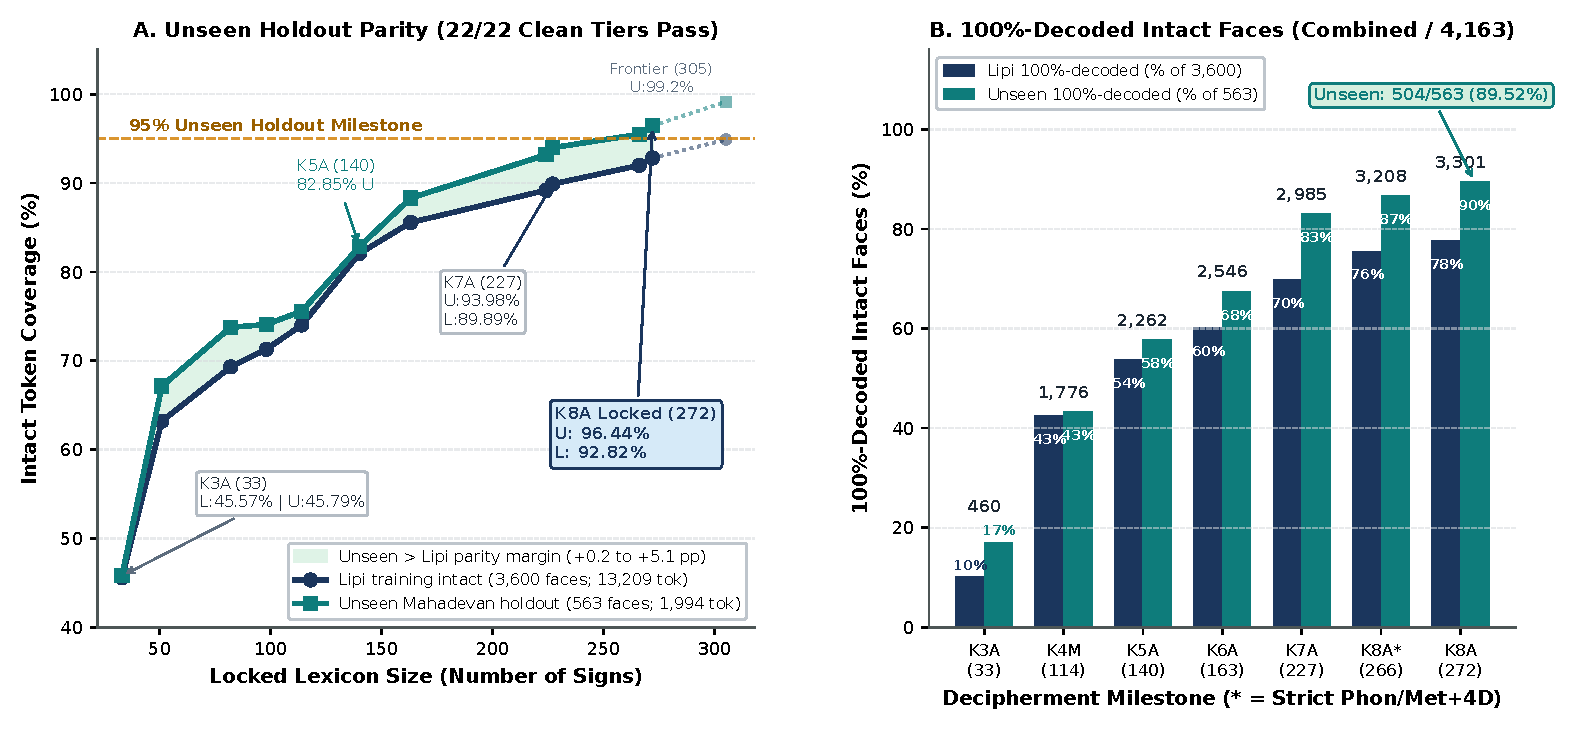
\includegraphics[width=\textwidth]{figures/fig1.pdf}
\caption{\textbf{Unseen holdout parity and whole-inscription decoding trajectory (33 $\to$ 272 locked signs).} \textbf{A}, Token coverage across cleanly crosswalked intact milestones on the Lipi training set (3,600 faces, 13,209 tokens) versus the unseen Mahadevan holdout (563 faces, 1,994 tokens). Across all 22/22 clean tiers, unseen holdout coverage strictly exceeds training coverage ($+0.22$ to $+5.06$ percentage points), crossing the 95\% unseen threshold at both the 266-sign strict tier (95.49\%) and the 272-sign locked lexicon (96.44\%). \textbf{B}, Share of 100\%-decoded intact faces rising from 460/4,163 (33 signs) to 3,301/4,163 (79.29\%) combined and 504/563 (89.52\%) on unseen Mahadevan inscriptions.}
\label{fig:coverage}
\end{figure}

\section{Six Strictly Disjoint Waves of Seven-Family Phonetic Identification}

\subsection{Programmatic 6-Wave Overlap Audit (15/15 Pairs Strictly Disjoint)}

Phonetic testing proceeded across six successive waves totaling \textbf{131 raw sign-tests} over \textbf{120 unique signs}: \textbf{Wave-1} (\texttt{Key \#2A}, 12 archaeologically anchored signs), \textbf{Wave-2} (\texttt{Key \#4B}, Top-30 high-frequency signs), \textbf{Wave-3} (\texttt{Key \#5A}, 13 Big-Six and Next-Nine bottlenecks), \textbf{Wave-4} (\texttt{Key \#6A}, 24 long-tail signs), \textbf{Wave-5} (\texttt{Key \#7A}, 27 untouched long-tail signs), and \textbf{Wave-6} (\texttt{Key \#8A}, 25 brand-new untouched long-tail signs with zero overlap against Waves 1--5 or \texttt{Key \#3A}).

Programmatic set-intersection auditing (\texttt{reproduce\_all\_keys.py}, Invariant~1) across all $\binom{6}{2} = 15$ wave pairs isolates every overlap: $\text{W1} \cap \text{W2} = \{861\}$ (1 sign), $\text{W2} \cap \text{W3} = \{060, 142, 240, 550, 798\}$ (5 Big-Six bottlenecks that scored 0/5 on \texttt{PhonEx} in W2 and were redesigned in W3), $\text{W2} \cap \text{W4} = \{142\}$ (1 sign), and $\text{W3} \cap \text{W4} = \{142, 527, 585, 595, 692\}$ (5 W3 holdouts re-tested in W4). All remaining 11 wave pairs—including every pair involving Wave-5 (27 signs) or Wave-6 (25 signs)—have strictly \textbf{zero overlap} ($\emptyset$). Additionally, Key~\#8A quarantined five post-hoc photo/corpus rescue signs (\texttt{921, 371, 645, 679, 267}) outside Wave-6 with zero unbiased discovery $P$-value claimed, and Wave-6 recorded zero duplicate \texttt{PhonEx} bridges.

Stripping all overlapping signs yields \textbf{115 strictly pairwise-disjoint signs} across six independent waves ($12 + 24 + 8 + 19 + 27 + 25$; 15/15 pairs disjoint), with five \texttt{W2}$\cap$\texttt{W3} bottlenecks excluded from all six waves in the conservative primary regime.

\subsection{6-Wave Meta-Analysis, Jackknife, Pooled Mega-Shuffle, and Daughter-Lexicon Audit}

Table~\ref{tab:meta6} and Figure~\ref{fig:meta} present the exact 6-wave Fisher combined probability \citep{fisher1932} ($\chi^2_{12} = -2\sum_{i=1}^6 \ln P_i$), Bonferroni-7 adjusted $P$, and empirical Stouffer $Z$ across all seven primary language families plus unedited \texttt{RawPDrav} (\path{work_data/key8c/combined_6wave_meta_stats.json}).

\begin{table}[htbp]
\centering
\caption{Six-Wave Strictly Pairwise-Disjoint 7-Family Meta-Analysis (115 Unique Signs: $12+24+8+19+27+25$, 15/15 wave pairs disjoint, $\text{df} = 12$, 5,000 cluster-preserving shuffles per wave).}
\label{tab:meta6}
\setlength{\tabcolsep}{3.5pt}
\resizebox{\textwidth}{!}{%
\begin{tabular}{@{}lrrrrrrrrrr@{}}
\toprule
Language Family (Single-HW) & W1 (12) & W2 (24) & W3 (8) & W4 (19) & W5 (27) & W6 (25) & $\chi^2_{12}$ & Fisher $P$ & Bonf-7 $P$ & $Z_{\text{emp}}$ \\
\midrule
\multicolumn{11}{l}{\textbf{Mode A: \texttt{PhonSt} (Phonemic Stem, 115 strictly disjoint signs)}} \\
\textbf{Proto-Dravidian (2-br)} & \textbf{9/12} & \textbf{23/24} & \textbf{5/8} & \textbf{14/19} & \textbf{14/27} & \textbf{7/25} & \textbf{70.95} & $\mathbf{2.13\times 10^{-10}}$ & $\mathbf{1.49\times 10^{-9}}$ & \textbf{+7.87} \\
\textit{Dravidian RawPDrav (audit)} & \textit{9/12} & \textit{22/24} & \textit{5/8} & \textit{12/19} & \textit{14/27} & \textit{6/25} & \textit{69.98} & $3.23\times 10^{-10}$ & $2.26\times 10^{-9}$ & \textit{+8.37} \\
Indo-Aryan (OIA) & 1/12 & 2/24 & 0/8 & 2/19 & 0/27 & 1/25 & 21.03 & 0.0499 & \textbf{0.3494} & +4.09 \\
Sumerian & 3/12 & 5/24 & 0/8 & 0/19 & 5/27 & 2/25 & 8.13 & 0.7749 & \textbf{1.0000} & +0.44 \\
Munda, Elamite, Akk., Bur. & 0/12 & 0/24 & 0/8 & 0/19 & 0/27 & 0/25 & 0.00 & 1.0000 & \textbf{1.0000} & $-0.42$ to $-0.17$ \\
\midrule
\multicolumn{11}{l}{\textbf{Mode B: \texttt{PhonEx} (Exact Phonemic Homophony, 115 strictly disjoint signs)}} \\
\textbf{Proto-Dravidian (2-br)} & \textbf{6/12} & \textbf{14/24} & \textbf{4/8} & \textbf{7/19} & \textbf{10/27} & \textbf{4/25} & \textbf{59.54} & $\mathbf{2.74\times 10^{-8}}$ & $\mathbf{1.92\times 10^{-7}}$ & \textbf{+7.55} \\
\textit{Dravidian RawPDrav (audit)} & \textit{6/12} & \textit{12/24} & \textit{4/8} & \textit{6/19} & \textit{10/27} & \textit{3/25} & \textit{59.66} & $2.60\times 10^{-8}$ & $1.82\times 10^{-7}$ & \textit{+7.95} \\
Indo-Aryan (OIA) & 0/12 & 2/24 & 0/8 & 1/19 & 0/27 & 0/25 & 11.06 & 0.5240 & \textbf{1.0000} & +2.08 \\
Sumerian & 1/12 & 1/24 & 0/8 & 0/19 & 1/27 & 1/25 & 2.38 & 0.9986 & \textbf{1.0000} & $-0.79$ \\
Munda, Elamite, Akk., Bur. & 0/12 & 0/24 & 0/8 & 0/19 & 0/27 & 0/25 & 0.00 & 1.0000 & \textbf{1.0000} & $-0.25$ to $-0.11$ \\
\bottomrule
\end{tabular}%
}
\end{table}

Wave-6 alone (\texttt{Key \#8A}, 25 ultra-rare long-tail signs) is transparently logged as individually non-significant (Dravidian \texttt{PhonEx} 4/25 vs 2.23 null, $z=+1.24, P=0.178$; \texttt{PhonSt} 7/25 vs 5.00 null, $z=+1.01, P=0.225$), reflecting the expected signal attenuation at the low-frequency tail (median $\le 12$ occurrences), where strict Key~\#7A gates promoted only 7/25 signs (\texttt{136, 792, 064, 411, 776, 111, 285}) and held 18/25 signs (including 3 Direct-only holds). Crucially, three independent robustness audits confirm that the 6-wave Proto-Dravidian signal is neither driven by any single wave nor an artifact of dictionary curation:
\begin{enumerate}
  \item \textbf{Leave-One-Wave-Out Jackknife (6/6 drops pass Bonferroni-7):} Dropping any single wave ($-\text{W1}$ through $-\text{W6}$) leaves Proto-Dravidian overwhelmingly significant on both \texttt{PhonSt} ($\chi^2_{10} = 53.91\text{--}67.97$, Bonf-7 $P = 7.66 \times 10^{-10}$ to $3.52 \times 10^{-7}$, Stouffer $Z_{\text{emp}} = +6.52\text{ to }+8.17$) and \texttt{PhonEx} ($\chi^2_{10} = 42.51\text{--}56.09$, Bonf-7 $P = 1.38 \times 10^{-7}$ to $4.27 \times 10^{-5}$), while best rival Indo-Aryan fails all 6/6 drops (Bonf-7 $P = 0.146\text{--}1.000$).
  \item \textbf{Single Pooled 115-Sign Mega-Shuffle (5,000 shuffles, no Fisher meta-pooling):} Evaluating all 115 strictly disjoint signs simultaneously yields \textbf{72/115} vs 38.89 null on \texttt{PhonSt} ($z = +6.08, P = 0.00020$, max null 61) and \textbf{45/115} vs 19.74 null on \texttt{PhonEx} ($z = +5.53, P = 0.00020$, max null 38); unedited \texttt{RawPDrav} yields 68/115 ($z=+6.59, P=0.00020$) and 41/115 ($z=+5.75, P=0.00020$). Every rival family fails Bonferroni-7 (\texttt{PhonSt} OIA 6/115 $P = 0.0160$ raw / Bonf-7 $P = 0.112$; \texttt{PhonEx} OIA 3/115 $P = 0.0772$; Sumerian $P = 0.371/0.863$; Munda, Elamite, Akkadian, Burushaski 0/115, $P = 1.000$).
  \item \textbf{Wider Daughter-Lexicon Sensitivity Audit (115 signs):} Replacing proto-reconstructions with much larger historical daughter lexicons confirms that rival failure is not a proto-dictionary artifact: \textbf{Turner OIA} (9,254 etyma \citep{turner1966cdial}) scores 7/115 \texttt{PhonSt} ($z=+1.84, P=0.073$) and 3/115 \texttt{PhonEx} ($z=+0.66, P=0.313$); \textbf{Campbell Santali Munda} (12,001 etyma \citep{campbell1899santali}) scores 3/115 \texttt{PhonSt} ($z=+0.61, P=0.321$) and 0/115 \texttt{PhonEx} ($P=1.000$); \textbf{Halloran Sumerian} (3,257 \citep{halloran2006}) scores 12/115 ($P=0.142$) and 4/115 ($P=0.547$); \textbf{Hinz--Koch Elamite} (2,437 \citep{hinz1987elam}) scores 0/115 ($P=1.000$). By contrast, all four Dravidian lexicons—\texttt{Dravidian 2-br} ($P=0.00020$), \texttt{RawPDrav} ($P=0.00020$), \texttt{Dravidian 2-Lang} (5,095; 80/115 \texttt{PhonSt} $z=+5.55$, 52/115 \texttt{PhonEx} $z=+5.25$, both $P=0.00020$), and \texttt{Tamil DEDR} (3,447; 81/115 \texttt{PhonSt} $z=+5.44, P=0.00020$; 47/115 \texttt{PhonEx} $z=+3.79, P=0.00060$)—clear Bonferroni-7 decisively. Ultra-Disjoint 114 signs (removing Key~\#3A sign \texttt{416}) likewise holds at $P = 8.49 \times 10^{-10}$ (\texttt{PhonSt}) and $P = 3.95 \times 10^{-7}$ (\texttt{PhonEx}).
\end{enumerate}

\begin{figure}[htbp]
\centering
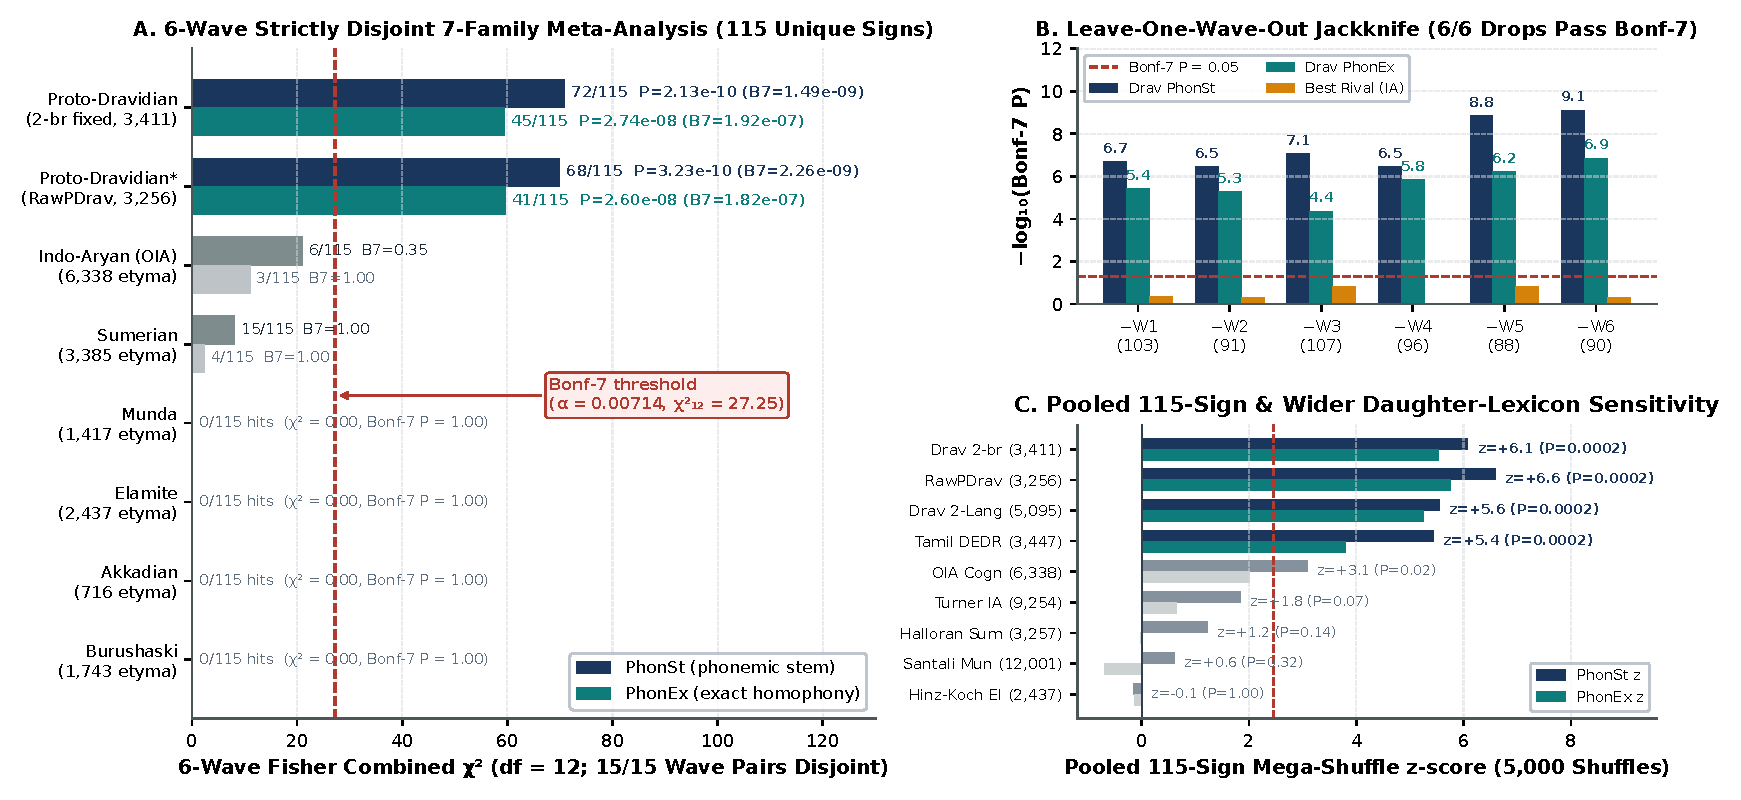
\includegraphics[width=\textwidth]{figures/fig2.pdf}
\caption{\textbf{Six-wave strictly pairwise-disjoint 7-family meta-analysis (115 unique signs) and robustness audits.} \textbf{A}, Fisher combined $\chi^2_{12}$ across all 7 primary Single-Headword language families plus unedited \texttt{RawPDrav}. Only Proto-Dravidian clears the Bonferroni-7 threshold ($\chi^2_{12} = 27.25$) on both \texttt{PhonSt} ($P = 2.13 \times 10^{-10}$) and \texttt{PhonEx} ($P = 2.74 \times 10^{-8}$). \textbf{B}, Leave-one-wave-out jackknife showing $-\log_{10}(\text{Bonf-7 } P)$ across all 6 wave drops; Proto-Dravidian passes 6/6 drops while Indo-Aryan fails 6/6. \textbf{C}, Single pooled 115-sign mega-shuffle and wider daughter-lexicon sensitivity (including 9,254-word Turner OIA and 12,001-word Santali Munda).}
\label{fig:meta}
\end{figure}

Core lexical locks established across Waves~1--6 include \texttt{740} \textit{*kuṭi} (`jar' $\leftrightarrow$ `house/lineage', DEDR 1651/1655), \texttt{090} \textit{*āḷ} (`man' $\leftrightarrow$ `manager'), \texttt{220} \textit{*mīṉ} (`fish' $\leftrightarrow$ `star', DEDR 4885/4876), \texttt{520} \textit{*vēḷ/*vēl} (`spear' $\leftrightarrow$ `lord'), \texttt{154} \textit{*kā} (`carrying-pole' $\leftrightarrow$ `guard'), \texttt{820/061} \textit{*kāl} (`wheel/leg' $\leftrightarrow$ `quarter/share'), \texttt{320} \textit{*paṭi} (`step' $\leftrightarrow$ `ration measure'), \texttt{705} \textit{*kalam/*kaḷam} (`ship/vessel/measure'), \texttt{400} \textit{*cikka} (`comb/junior'), \texttt{390/405} \textit{*tai} (`plant' $\leftrightarrow$ `weave'), \texttt{590} \textit{*mūṭai} (`bale'), \texttt{615} \textit{*accu} (`grid/plot'), \texttt{845} \textit{*vari} (`hatched' $\leftrightarrow$ `tax/levy'), \texttt{142} \textit{*kōl} (`staff' $\leftrightarrow$ `smith/gauge-rod', $P = 2.43 \times 10^{-61}$ before \texttt{615/617}), \texttt{595} \textit{*mūṭai-vari} (`bale-tax'), \texttt{482} \textit{*kō} (`mountain' $\leftrightarrow$ `king', $P = 6.43 \times 10^{-25}$ before \texttt{740/752}), \texttt{630/632} \textit{*kūṭu} (`granary/depot'), \texttt{585} \textit{*paḷḷi} (`citadel hall', $P = 2.72 \times 10^{-51}$), \texttt{621} \textit{*aṟai/*paṭi} (`3-compartment chamber'), \texttt{347/341} \textit{*mā} (`deer' $\leftrightarrow$ `great'), \texttt{388/382} \textit{*aracu/*āku} (`royal pipal emblem'), \texttt{285} \textit{*cūṭu} (`crest/bundle', unlocking Gonur Depe \texttt{4155.1} to 8/8 = 100\%), and \texttt{645} \textit{*kaṭa/*kaṭam} (`cross/passage-tax tally').

\section{Internal Grammar, Exogenous Deconflation, and the Dholavira Signboard}

\subsection{Head-Final Syntax, Diacritic Operators, Doubles, and Catalogue Compression}

Six distributional levers establish the script's internal morphosyntax independently of phonetic guesses:
\begin{itemize}
  \item \textbf{Head-final compound order (\texttt{Keys \#3A, \#4B}):} Modifier-before-Head / Possessor-before-Possessed order holds at \textbf{93.5\%} (331/354, $P = 0.0040$) in Lipi and \textbf{98.4\%} (61/62, $P = 0.0050$) on unseen Mahadevan texts (75.8\% tokens / 71.0\% unseen compound types across 49 signs, $P = 0.0010$), matching Proto-Dravidian SOV head-final typology.
  \item \textbf{Four cross-base diacritic operators (\texttt{Keys \#4A, \#6A, \#7A}):} \texttt{cage\_4corners} ($k=8$ pairs, $\Delta\text{F400}$ $P = 0.0002$; inverse proof \texttt{175 $\to$ 176} $P_{\text{joint}} = 0.00240$), \texttt{side\_brackets} ($k=6$, $\cos_L - \cos_R$ $P = 0.0054$; unlocking \texttt{048/049} \textit{*[BRACKET]-ēḻ}, $P = 3.52 \times 10^{-15}$), \texttt{multi\_stroke\_inside} ($k=10$, $\cos_L$ $P = 0.0114$), and photo-verified horizontal hatching \textit{*vari} ($k=5$ pairs, mean $\cos_L - \cos_R = +0.489$ vs $+0.159$ null, $P = 0.0422$, cleanly separated from diagonal-veined botanical pipal-leaf control \texttt{384 $\to$ 388}, $+0.050$). Nineteen graphic ligatures match 2-branch DEDR stems at 18/19 ($P = 0.0026$) and \texttt{PhonEx} 14/19 ($P = 0.0068$).
  \item \textbf{Postposition \texttt{060}, precinct header \texttt{692}, and Rank \#1 doubles (\texttt{Keys \#5A--\#7A}):} Medial postposition \texttt{060} (\textit{*-uḷ/*-iṉ}, 94.4\% medial, $\Delta H_{R-L} = +1.635$ bits) stands in near-total complementary distribution with numeral \texttt{002} across place/time headers (\texttt{920, 550, 692}) vs weight/share headers (\texttt{861, 817}): \textbf{112:6 vs 1:267} ($\text{OR} = 4{,}984, P = 8.80 \times 10^{-89}$) in Lipi and a zero-exception \textbf{16:0 vs 0:29} ($P = 1.55 \times 10^{-12}$) on unseen Mahadevan texts. Precinct header \texttt{692} locks identically (\textbf{40:0 vs 1:296}, $P = 2.93 \times 10^{-51}$; unseen \textbf{9:0 vs 0:29}, $P = 6.13 \times 10^{-9}$). Three catalog doubles lock at Rank~\#1/150 ($P = 0.0002$): \texttt{617 == 615-615}, \texttt{821 == 820-820}, and \texttt{091 == 090-090}.
  \item \textbf{Distributional allograph compression (\texttt{Key \#4D}):} Contextual JSD and 5-fold Brown class perplexity \citep{brown1992} compress the 638-sign Lipi inventory to 541 (pure) / 522 (pure+workshop) signs, lowering perplexity from 5.3654 to \textbf{5.3016 bps} ($z = -10.72, P = 0.0005$) in Lipi and from 5.4884 to \textbf{5.4093 bps} ($z = -4.12, P = 0.0110$) on unseen holdout texts, while catching 67 visually similar false mergers that worsen perplexity (5.3858 bps).
\end{itemize}

\subsection{Exogenous Artifact-Class Deconflation of Lipi \texttt{824} (\texttt{Key \#8A})}

Direct carved-stone photograph auditing (\texttt{Key \#7D} and \texttt{Key \#8A}, inspecting 27 additional sign sheets beyond the initial 14 holdouts) exposed a major catalogue conflation under Lipi \texttt{824} (32 Lipi rows, 0 unseen). Splitting \texttt{824} strictly by \textit{exogenous artifact class}—never by token position—cleanly separates two unrelated graphemes (\texttt{work\_data/key8a/m284\_824\_analysis.json}):
\begin{itemize}
  \item \textbf{\texttt{824a} (seals, 10 all / 7 intact, 6 photo-verified):} A vertically divided lozenge (\texttt{M267}), 100\% initial (10/10) and immediately preceding \texttt{002} in 9/10 cases ($P = 2.86 \times 10^{-7}$). Its clean exogenous distributional profile matches locked \texttt{817} \textit{*kāṇam} at $\cos_{\text{mean}} = \mathbf{0.9973}$ ($\cos_L = 0.9991, \cos_R = 0.9954$) and \texttt{861} \textit{*kāṇam} at $\mathbf{0.9705}$.
  \item \textbf{\texttt{824b} (Harappa miniature tablets, 22 all / 18 intact, 8 photo-verified, including reversed \texttt{H-2085}):} The 4-quartered diamond/wheel (\texttt{M284}, \textit{*nāl-kāṇam}), showing $\cos_{\text{mean}} = \mathbf{0.0000}$ against \texttt{824a}, locking after \texttt{892} (\texttt{413-892-824b}, 12/18, $\text{OR} = 467\times, P = 2.98 \times 10^{-24}$) and \texttt{032} ($P = 0.0033$, shared with \texttt{877} \texttt{032-877}, $P = 1.47 \times 10^{-10}$), while carved-stone photos of \texttt{880} (\texttt{M-6\_a}) reveal an explicit diamond-enclosing-wheel ligature (\texttt{861+820} \textit{*kāṇam-*kāl}, $\cos_{\text{mean}} = 0.9273$ vs \texttt{817}). The blind seals-vs-tablets separation of \texttt{824a} vs \texttt{824b} achieves $\text{OR} = \mathbf{945.0\times}$ ($P = 0.00020$).
\end{itemize}

\subsection{The Dholavira North Gate Signboard (\texttt{Lipi 144.1}): \texttt{8/10} Strict, \texttt{9/10} Corpus, \texttt{10/10} Glossed}

Auditing the monumental $\sim$3.0~m white gypsum-inlay Dholavira North Gate Signboard (\texttt{Lipi 144.1}) directly against Bisht's (2015) official excavation photographs, line drawings, and ASI field card (\texttt{24.03.95}) \citep{bisht2015} upgrades the inscription from 7/10 (\texttt{Key \#7D}) to \textbf{8/10 strict phonetic tokens locked}, \textbf{9/10 with corpus \texttt{645}}, and \textbf{10/10 glossed with architectural \texttt{611}} (Figure~\ref{fig:dholavira}; \path{work_data/key8a/dholavira_signboard_audit_v2.json}):
\begin{enumerate}
  \item \textbf{Orientation and \texttt{821} expansion:} Fallen face-down from the 3.5~m North Gate lintel into the Western Chamber, flipping the board upright places \texttt{820-611-388} at right for standard Harappan R$\to$L reading, independently confirmed by \texttt{820}'s 71.5\% initial rate, \texttt{798}'s 72.2\% medial/1.9\% final rate, the exact Gujarat opening parallel \texttt{820-611} on Lothal \texttt{L-116} \citep{rao1979lothal}, and Key~\#5A's Rank~\#1 double \texttt{821 == 820-820} (\textit{*iru-kāl}).
  \item \textbf{Sign \#3 (\texttt{388}, \texttt{M327}) — Royal Pipal Emblem Lock:} Carved-stone sheets confirm a chevron-veined pipal (\textit{Ficus religiosa}) leaf with twin top buds matching locked plain pipal-leaf \texttt{384} ($\cos_{\text{mean}} = 0.8343$), locking tightly into \texttt{388 $\to$ 443} ($\text{OR} = 723\times, P = 1.47 \times 10^{-11}$), \texttt{585 $\to$ 388} ($P = 1.12 \times 10^{-5}$), and \texttt{388 $\to$ 740} ($P = 7.13 \times 10^{-7}$). Crucially, \texttt{Key \#8A} verified that \textbf{both} DEDR~202 \textit{*aracu} (`pipal') and DEDR~201 \textit{*aracaṉ} (`king') sit in both 2-branch \texttt{FIX} and \texttt{RAW} Proto-Dravidian (failing single-headword exact match solely due to masculine \textit{-aṉ}).
  \item \textbf{Sign \#6 (\texttt{645?}, \texttt{M137}) — Corpus Lock with Transparent In-Situ Caveat:} Corpus sign \texttt{645} (27C/5N) locks via \texttt{104 $\to$ 645} ($P = 2.14 \times 10^{-15}$), \texttt{645 $\to$ 590} ($P = 4.31 \times 10^{-9}$), and FIX-only 2-branch \texttt{PhonSt} DEDR~1109 \textit{*kaṭa} (`pass through, cross') $\leftrightarrow$ 1113 \textit{*kaṭam} (`duty, tax, tribute'; \texttt{RAW} misaligns \texttt{eid=1109} onto \texttt{cid=5091}), while slender Y-fork \texttt{064} is visually ruled out. Because Bisht Fig.~8.4 shows five gypsum strips in an inverted-V+apex amid documented late-Harappan disturbance (19 loose stone-paste strips on ASI card \texttt{24.03.95}), Sign~\#6's identification on \texttt{144.1} is transparently flagged (8/10 strict vs 9/10 with corpus \texttt{645}).
  \item \textbf{Sign \#2 (\texttt{611}, \texttt{M256}) — Architectural Portal Lock:} All 6/6 Lipi findspots are monumental or giant-seal administrative contexts (Dholavira North Gate, Harappa Mound~F Granary \texttt{H-3} 2,767~mm$^2$, Lothal \texttt{L-116} \texttt{820-611}, Mohenjo-daro \texttt{M-56} 1,176~mm$^2$, \texttt{H-1076} with \texttt{820}; co-occurrence with \texttt{820} $\text{OR} = 23.2\times, P = 0.0013$). Its architectural gate-lintel/canopy meaning is locked while its exact single Proto-Dravidian root remains open between 2-branch DEDR~3694 \textit{*nukam} (`protecting bar') and 1663 \textit{*kuṭai} (`canopy').
\end{enumerate}

\begin{figure}[htbp]
\centering
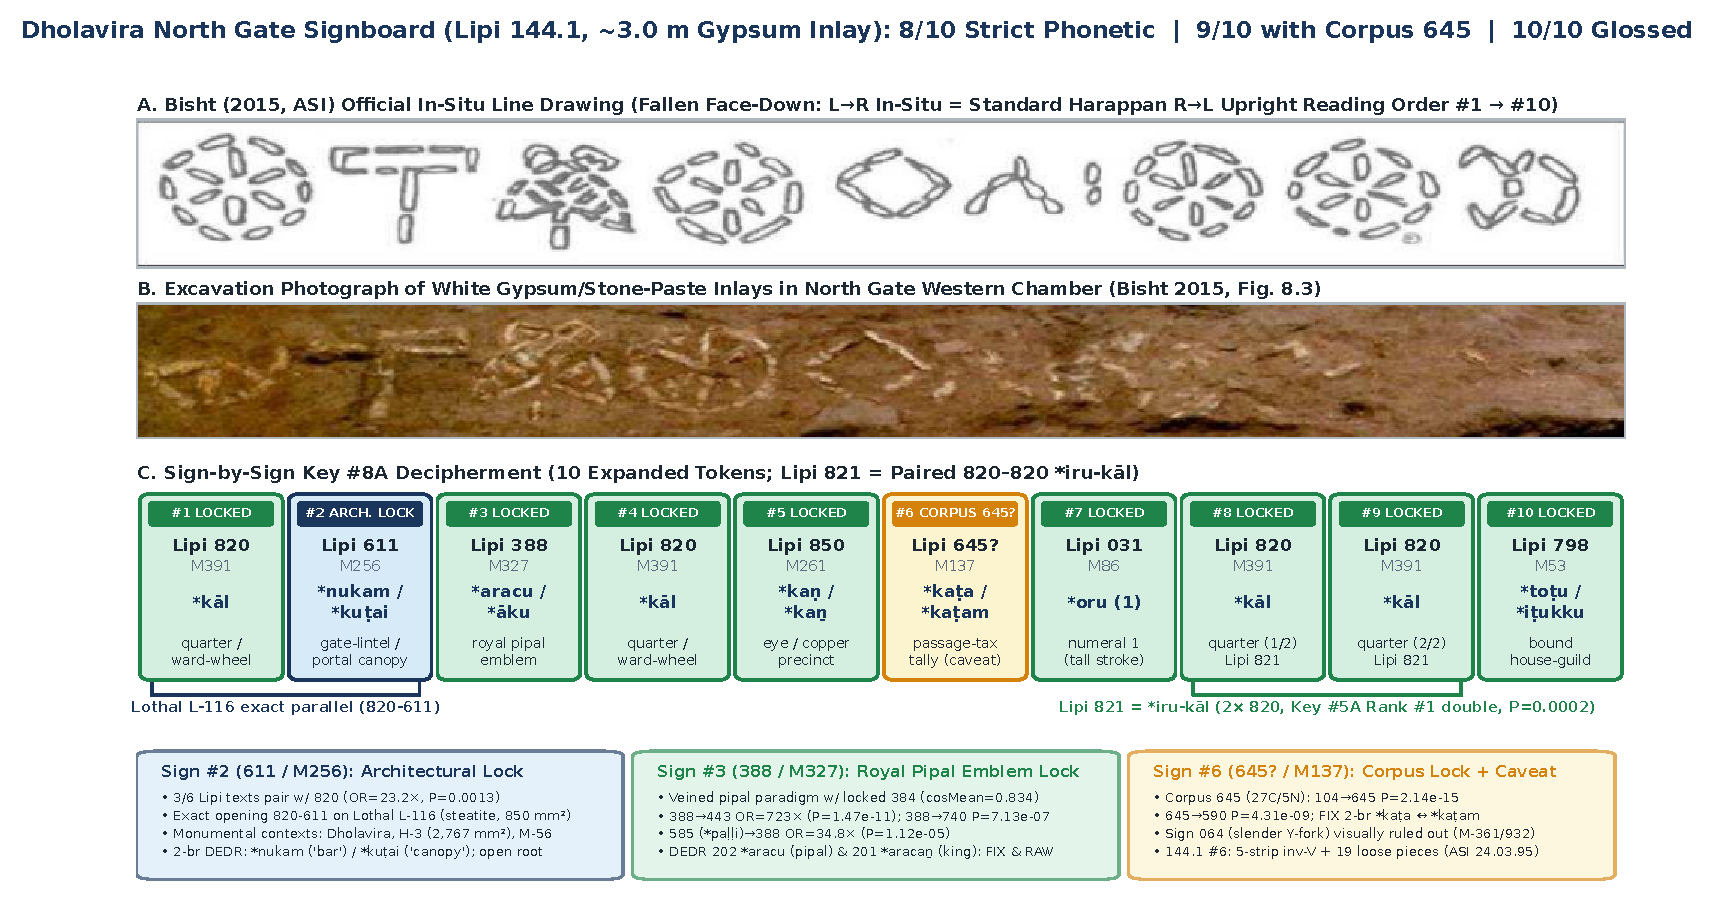
\includegraphics[width=\textwidth]{figures/fig3.pdf}
\caption{\textbf{Dholavira North Gate Signboard (\texttt{Lipi 144.1}, $\sim$3.0~m white gypsum inlay).} \textbf{A}--\textbf{B}, Official Bisht (2015, ASI) in-situ line drawing and excavation photograph. \textbf{C}, Ten-tile sign-by-sign breakdown under Key~\#8A: 8/10 strict phonetic locks (green), 9/10 including corpus \texttt{645} \textit{*kaṭa/*kaṭam} with physical-disturbance caveat (amber), and 10/10 glossed with architectural portal lock \texttt{611} (blue), showing the exact Lothal \texttt{L-116} (\texttt{820-611}) parallel and Rank~\#1 double \texttt{821 = 820-820} (\textit{*iru-kāl}).}
\label{fig:dholavira}
\end{figure}

\section{Diachronic Continuity: Four-Tier Sangam Epigraphy and Chola Metrology}

To test whether decoded Harappan values survive across the $\sim$1,500--2,000-year gap into Old Tamil Sangam literature, Early Tamil-Brahmi epigraphy \citep{mahadevan2003ete}, and Chola administrative records \citep{subbarayalu2012} without circularity, \texttt{Key \#4C}, \texttt{Key \#7B}, and \texttt{Key \#8B (Test 8B-1)} benchmark the frozen 272-sign lexicon across four nested tiers (5,000 permutations each; Table~\ref{tab:sangam} and Figure~\ref{fig:sangam_multiface}A):

\begin{table}[htbp]
\centering
\caption{Four-Tier Zero-Circularity Sangam / Tamil-Brahmi Compound Validation (272-Sign Lexicon, 1,004 Lipi $\ge 2$ bigrams; 5,000 permutations) and Volumetric Metrology Benchmark (\texttt{Test 4C.3}).}
\label{tab:sangam}
\setlength{\tabcolsep}{4pt}
\resizebox{\textwidth}{!}{%
\begin{tabular}{@{}lrrrrrrr@{}}
\toprule
Tier / Control Lexicon (272 Signs) & Target Size & Obs.\ Words & Null Mean & Perm $z$ & Perm $P$ & Lipi Mass & Unseen Mass \\
\midrule
\textbf{Tier 1: Frozen Pure-Dravidian} & 170 & \textbf{38} & 15.05 & \textbf{+5.56} & \textbf{0.00020} & 988 & 160 \\
\textbf{Tier 2: Expanded Pure-Dravidian (Lipi $\ge 2$)} & 220 & \textbf{52} & 18.69 & \textbf{+6.89} & \textbf{0.00020} & \textbf{1,202} & \textbf{186} \\
\quad Tier 2 Combined ($\text{Lipi+New} \ge 2$) & 220 & \textbf{54} & 21.51 & +6.19 & 0.00020 & 1,207 & 198 \\
\quad Tier 2 Wave-5/6 Novel ($\ge 1$ new sign) & 220 & \textbf{16} & 5.86 & \textbf{+5.00} & \textbf{0.00020} & 231 & 27 \\
\quad Tier 2 Wave-5/6 Novel (both new signs) & 220 & \textbf{2} & 0.09 & +6.20 & 0.00540 & 18 & 2 \\
Tier 2 Quarantined Prakrit Control & 30 & \textbf{0} & 0.00 & 0.00 & 1.00000 & 0 & 0 \\
Tier 2 MW-Verified Indo-Aryan Rival & 140 & 16 & 9.23 & +2.47 & 0.02280 & 367 & 59 \\
Tier 2 Halloran Ur~III Sumerian Rival & 114 & 4 & 6.78 & $-1.10$ & 0.92282 & 223 & 45 \\
\midrule
\textbf{Tier 3: Non-Numeral Lexical-Only Dravidian} & 220 & \textbf{34} & 7.06 & \textbf{+7.72} & \textbf{0.00020} & \textbf{857} & \textbf{133} \\
Tier 3 Lexical-Only MW Indo-Aryan & 140 & 8 & 4.03 & +1.67 & 0.08098 & 236 & 45 \\
Tier 3 Lexical-Only Ur~III Sumerian & 114 & 3 & 5.96 & $-1.20$ & 0.93641 & 218 & 45 \\
\midrule
\textbf{Tier 4: Uncurated DEDR Tamil (Exact Phon.)} & 14,206 & \textbf{11} & 5.29 & \textbf{+2.56} & \textbf{0.01920} & 249 & 27 \\
\quad Tier 4 Uncurated DEDR Tamil (Pairs) & 14,206 & 22 pairs & 6.80 & +4.57 & \textbf{0.00100} & 249 & 27 \\
\midrule
\multicolumn{8}{l}{\textbf{Volumetric Metrology Benchmark (\texttt{Test 4C.3}, 5,000 random ladders; cup counts $\{1,2,3,4,6\}$ = 437/438 = 99.77\%):}} \\
\textbf{Old Tamil / Chola \texttt{(8, 4, 3)} Ladder} & 3/3 steps & Super 12 & Lit.\ 0.890 & \textbf{+5.30} & \textbf{0.00040} & \multicolumn{2}{r}{Composite 2.887} \\
Ur~III Sumerian / Vedic-Arthaśāstra (shifted, base) & 0--1/3 & 30 / 64 / 16 & 0.09--0.65 & $-0.64$--+0.58 & 0.256--0.773 & \multicolumn{2}{r}{1.000--1.386} \\
\bottomrule
\end{tabular}%
}
\end{table}

Key zero-circularity findings include:
\begin{itemize}
  \item \textbf{52 attested pure-Dravidian compounds (0 Prakrit loans):} Scaling from 163 to 272 signs expands attested Old Tamil compounds from 38 to \textbf{52} ($z = +6.89, P = 0.00020$; random DEDR draw $z = +27.81, P = 0.00020$), with \textbf{45} distinct compounds replicated in unseen Mahadevan holdout texts (203 tokens). Newly locked Wave-5/6 signs add \textbf{16} novel attested compounds (\textit{aracukuṭi}, \textit{aracuvēḷ}, \textit{iṟaimūṭai}, \textit{kuṭikkuṭai}, \textit{kuṭiyaṟai}, \textit{kūṭṭukkaṭṭu}, \textit{kūṭṭukkuṭi}, \textit{muppāl}, \textit{mālaikkuṭi}, \textit{mūṭaikkuṭi}, \textit{nāṭṭukkuṭi}, \textit{nāṭṭumeṭṭu}, \textit{paḷḷikkuṭi}, \textit{paḷḷiyāḷ}, \textit{taṇṭukkaṭam}, \textit{toṭṭikkuṭi}; $z = +5.00, P = 0.00020$), including two with \textit{both} signs newly locked in Waves 5--6 (\textit{nāṭṭumeṭṭu}, \textit{paḷḷiyāḷ}; $z = +6.20, P = 0.0054$).
  \item \textbf{Numeral-calque elimination (Tier~3):} Stripping all numerals collapses Indo-Aryan to non-significance (8 words vs 4.03 null, $z = +1.67, P = 0.081$) and Ur~III Sumerian to negative ($z = -1.20, P = 0.936$), while Proto-Dravidian strengthens to \textbf{34} non-numeral lexical compounds vs 7.06 null ($z = +7.72, P = 0.00020$; Lipi mass 857 vs 70.0, $z = +10.57$; unseen mass 133 vs 11.3, $z = +9.98$).
  \item \textbf{Zero-curation automated dictionary proof (Tier~4):} Matching 1,004 Indus bigrams blindly against the uncurated 14,206-word DEDR Tamil dictionary passes exact-phoneme permutation on words (11 vs 5.29, $P = 0.0192$), pairs (22 vs 6.80, $P = 0.0010$), Lipi mass ($P = 0.0294$), and unseen mass ($P = 0.0340$).
  \item \textbf{Double account-order reversal and Chola metrology (\texttt{Key \#4C}):} Indus inscriptions place \texttt{NUM + THING} in 87.9\% (632/719) of Lipi and 98.9\% (471/476) of Mahadevan commodity counts, yet reverse to \texttt{MEAS + NUM} in 82.6\% (218/264) of Lipi and 84.0\% (142/169) of Mahadevan capacity measures (Fisher $P = 7.54 \times 10^{-98}$ Lipi, $P = 3.47 \times 10^{-107}$ Mahadevan)—matching Tamil-Brahmi on 6/6 syntax axes ($\cos = 0.899$) while beating Prakrit-Brahmi ($P = 0.0100$) and Ur~III Sumerian ($\cos = -0.427, P = 0.00020$). Cup counts (\texttt{700}) hit $\{1,2,3,4,6\}$ in 437/438 instances (0 fives), locking the Chola \texttt{(8, 4, 3)} ladder ($z = +5.30, P = 0.00040$; Table~\ref{tab:sangam}).
\end{itemize}

\begin{figure}[htbp]
\centering
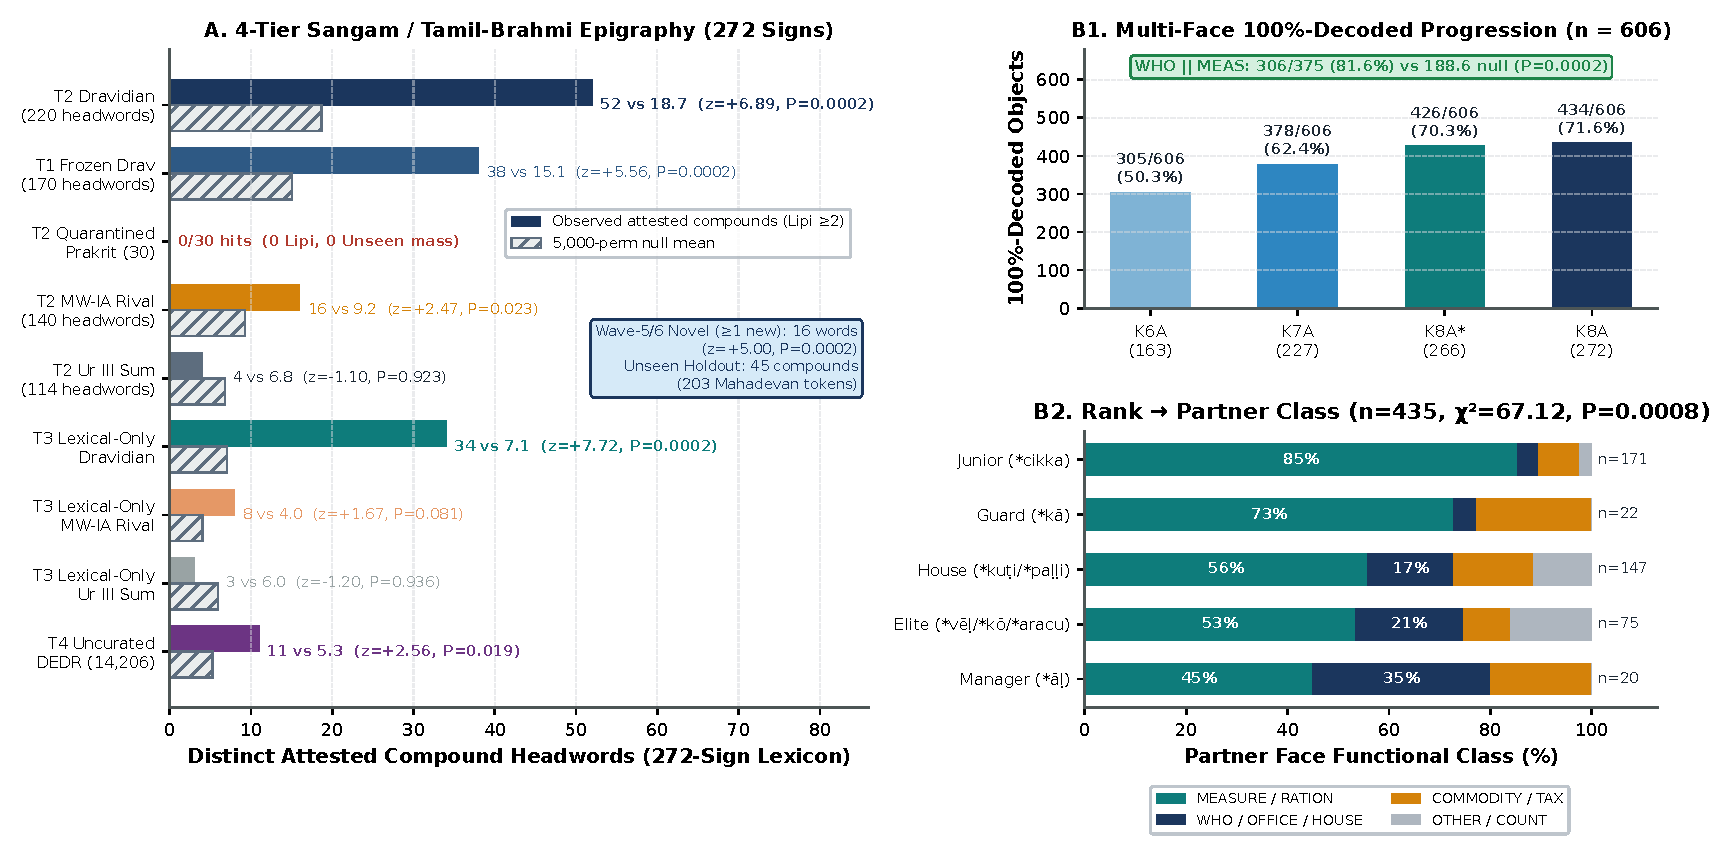
\includegraphics[width=\textwidth]{figures/fig4.pdf}
\caption{\textbf{Zero-circularity 4-tier Sangam epigraphy and whole-object multi-face accounting (272 signs).} \textbf{A}, Observed vs 5,000-permutation null headwords across Tiers~1--4: 52 attested pure-Dravidian compounds ($z = +6.89, P = 0.0002$) and 34 non-numeral lexical-only compounds ($z = +7.72, P = 0.0002$) versus 0/30 Prakrit loans, null lexical-only MW-IA ($P = 0.081$), and negative Ur~III Sumerian ($P = 0.936$). \textbf{B1}, Whole-object 100\%-decoded multi-face progression reaching 434/606 (71.6\%) intact objects, with 81.6\% \texttt{WHO$\parallel$MEASURE} complementarity ($P = 0.0002$). \textbf{B2}, Recipient rank strongly predicts partner-face functional class ($\chi^2 = 67.12, P = 0.0008$).}
\label{fig:sangam_multiface}
\end{figure}

\section{External Validation: Multi-Face Accounting, Blind Archaeology, Overseas Frontier, and External Bridges}

\subsection{Whole-Object Multi-Face Bureaucratic Accounting (\texttt{Key \#8B}, Test 8B-3)}

Scaling the 921 linked multi-face objects (824 Lipi, 97 unseen Mahadevan; 606 intact, 558 batch-deduplicated) to the 272-sign lexicon raises 100\%-decoded whole multi-face objects from 305 (163 signs) and 378 (227 signs) to \textbf{434/606 (71.62\%)} (\textbf{426} strict 266-sign; 395 batch-deduplicated: 369 tablets, 38 seals, 14 copper tablets, 8 tags/sealings, 3 pots, 2 other; Figure~\ref{fig:sangam_multiface}B1--B2):
\begin{itemize}
  \item \textbf{Double-entry \texttt{WHO$\parallel$MEASURE} complementarity:} Among batch-deduplicated 2-face objects in the \texttt{WHO} vs \texttt{MEASURE} pool ($n = 375$), \textbf{306/375 (81.60\%)} pair one \texttt{[WHO/OFFICE/HOUSE]} face with one \texttt{[MEASURE/RATION]} face (58 \texttt{WHO+WHO}, 11 \texttt{MEAS+MEAS}) versus 188.63 re-pairing null and 180.56 pooled-pair null (both $P = 0.00020$).
  \item \textbf{Rank governs voucher vs inter-house contract class:} Across 435 batch-deduplicated ranked multi-face objects, recipient rank strongly predicts partner-face class ($\chi^2 = 67.12$ vs 34.26 null, $P = 0.00080$): Junior (\textit{*cikka}, 146/171 = 85.4\%) and Guard (\textit{*kā}, 16/22 = 72.7\%) pair with ration vouchers, whereas Elite (\textit{*vēḷ/*talai/*kō/*aracu}, 16/75 = 21.3\%) and Manager (\textit{*āḷ}, 7/20 = 35.0\%) pair heavily with second institutional houses. Commodity-to-measure-unit coupling also passes ($\chi^2 = 100.33, P = 0.0492$), whereas cup counts per voucher stay flat at $\sim$3~cups across ranks (Kruskal--Wallis $H = 3.15, P = 0.529$, honest null).
\end{itemize}

\subsection{Blind Physical Archaeology and 600-Year Stratigraphic Stability (\texttt{Keys \#5B--\#8B})}

Using 5,000-permutation stratified tests on physically deduplicated objects (1,070 measured square seals, corpus median 645.2~mm$^2$; 3,212 city-assigned events; 2,589 dated events; Figure~\ref{fig:arch_bridges}):
\begin{itemize}
  \item \textbf{Carved square-seal area tracks decoded rank:} Controlling simultaneously for inscription length (OLS $+0.1102\ \log\text{mm}^2$/sign) and city, pre-registered \textbf{Elite} titles ($n = 469$, median \textbf{778.4~mm$^2$}) decisively exceed \textbf{Subordinate} roles ($n = 158$, median \textbf{531.2~mm$^2$}) by $+0.211\ \log\text{mm}^2$ ($P = 0.00020$; strictly excluding structural \texttt{692}: $P = 0.00020$). Individual giant-seal locks include \texttt{595} \textit{*mūṭai-vari} (1,258.5~mm$^2$, $P = 0.00460$), \texttt{692} \texttt{[PRECINCT-HEADER]} (976.5~mm$^2$, $n=25$, $P = 0.00300$), and \texttt{*ammā} (852.6~mm$^2$, $P = 0.0238$), versus compact \texttt{*cikka} (521.0~mm$^2$, $P = 0.00080$) and \texttt{*kā} (541.1~mm$^2$, $P = 0.0230$).
  \item \textbf{Blind object-class and site specialization:} City$\times$Domain specialization reaches $\chi^2 = 205.00$ ($P_{\text{obj}} = 0.00160$; coastal ports \textit{*pāy} $\text{OR} = 6.33, P = 0.0060$; Harappa granary/ration $\text{OR} = 6.74, P = 0.00020$), and the textile-guild signature \textit{*mūṭai-tai-kuṭi} spans 12 sites linking Harappa (\texttt{H-134}), Kish (\texttt{1971.1}), and Gonur Depe (\texttt{4155.1}). Following 18/23 confirmed Wave-4 object/site predictions (\texttt{Key \#7B}), \texttt{Key \#8B} tests 32 new Wave-5/6 predictions and confirms \textbf{19/32 strictly at $P < 0.05$} (plus 2 trends at $P < 0.09$; 11 honest nulls), including \texttt{824a/b} seals vs Harappa tablets ($\text{OR} = 945.0\times, P = 0.00020$), \texttt{167/868} Harappa tablets (22/22, $\text{OR} = 150.8\times, P = 0.00020$), \texttt{391} \textit{*toṇṭu} bronze/copper tools ($\text{OR} = 145.6\times, P = 0.00020$), \texttt{924} \textit{*vari-tiṅkaḷ} foreign trade ($\text{OR} = 46.3\times, P = 0.00040$), \texttt{890} \textit{*vil} Kalibangan sealings ($\text{OR} = 44.1\times, P = 0.00020$), \texttt{095} copper tablets ($\text{OR} = 38.1\times, P = 0.00020$), \texttt{243} hatched fish on seals (15/15, $\text{OR} = 26.5\times, P = 0.00080$), \texttt{621} \textit{*aṟai} seals (25/26, $\text{OR} = 21.4\times, P = 0.0010$), \texttt{880} package sealings ($\text{OR} = 14.2\times, P = 0.0030$), and \texttt{585} \textit{*paḷḷi} copper tablets ($\text{OR} = 13.2\times, P = 0.00020$).
  \item \textbf{600-year stratigraphic invariance:} Across 2,589 dated events (Early 344, Middle 1,490, Late 755), the positive chronological detector fires right on target (Harappa inscription-only bar seals \texttt{SEAL:I} rise $27.3\% \to 25.3\% \to 38.8\%$, $r = +0.1256, P = 0.0366$). Against this verified detector, \textbf{24/24} Wave-5/6 sign families, \textbf{21/21} Key~\#5 institutional markers, and 272-sign 100\%-decoded intact coverage ($70.17\% \to 69.79\% \to 67.75\%, P = 0.351$) remain completely flat across 600 years (Figure~\ref{fig:arch_bridges}B2).
\end{itemize}

\subsection{Overseas Frontier and Five Independent External Bridges (\texttt{Keys \#1--\#4E, \#8D})}

Beyond the Indus heartland, decoded values survive across both overseas trade frontiers \citep{gadd1932,laursen2010,steinkeller1982} and five orthogonal archaeological bridges audited in \texttt{Key \#8D} (\texttt{work\_data/key8d/key8d\_summary.json}):
\begin{enumerate}
  \item \textbf{Overseas frontier (\texttt{Keys \#1, \#2B, \#2C, \#3B, \#4E}):} Gulf round seals preserve the mainland right-facing bull compass (23/24 = 95.8\%) while carving positive-cut scripts at $3.77\times$ the mainland rate ($P = 0.0309$; flipping 3--4 seals lifts Bahrain/Failaka bigram alignment from 28.7\% to 67.6--71.3\% and Ur from 63.5\% to 81.6\%) and encode Mesopotamian personal names logographically ($z = +67.56, P = 0.0005$), independently matched by Ur~III sea-trader tablets (\texttt{UET 3}) carrying 68.8\% Nanna/Suen Moon names vs 8.5\% at Girsu ($\text{OR} = 23.74, P = 8.03 \times 10^{-16}$). BMAC Central Asian square seals preserve mainland head-final syntax (8/9 = 88.9\% ordered bigrams, 0/13 \texttt{MAN}-initial) vs Gulf/Iranian \texttt{MAN}-initial formulas ($P = 0.0002$), while the Harappan 13.65~g weight locks $1/100$ of the Dilmun mina ($P = 0.0068$).
  \item \textbf{Mohenjo-daro copper tablet pictorial bilinguals (\texttt{Key \#8D.1}):} Copper tablets decode at 95.2\% of clean obverse tokens (852/895). Nine picture-face signs are 92.3\% exclusive to copper tablets (24/26, Fisher $P = 1.02 \times 10^{-30}$; rarity-matched perm $z = +25.64, P = 0.00020$). Critically, locked tusk/horn sign \texttt{923} (\textit{*maruppu}) appears on \textbf{11/11} elephant copper tablets in Lipi (Fisher $P = \mathbf{3.81 \times 10^{-16}}$; 6/7 in M77, $P = 7.67 \times 10^{-8}$) yet sits on unicorn seals elsewhere; locked deer sign \texttt{341} (\textit{*mā}) pairs with the \texttt{503-615-740} stag-tablet twin ($P = 0.0040$ among pic-signs); deduplicated obverse-emblem pairing (\texttt{923}, \texttt{407}) passes at $z = +4.21, P = 0.00040$; and \texttt{176} $\leftrightarrow$ \texttt{384} frame-swapping holds out-of-copper ($P = 0.0070$).
  \item \textbf{Meluhha cuneiform loanword endemism stratification (\texttt{Key \#8D.2}):} Testing Mesopotamian Meluhha trade terms \citep{parpola1975meluhha,witzel1999substrate} by biogeographic endemism shows \texttt{Dravidian\_2Lang} hitting 3/5 strict-Indus \texttt{S1} items ($P = 0.0158$) and 4/9 \texttt{S1+S2} items ($P = 0.0136$) versus 0/6 native Sumerian controls and 1/10 Zagros transit minerals ($P = 0.164$), while all six rivals plus Turner OIA and Santali Munda score 0 hits ($P = 1.000$); strict 2-branch Dravidian ($P = 0.349$) and Bonferroni-7 ($\alpha = 0.00714$) remain honestly logged as null.
  \item \textbf{Pre-city Period 1--2 continuity (\texttt{Key \#8D.3}):} Early Harappan pre-city pottery/seals (2800--2600 BCE, $n=38$) decode at \textbf{83.64\%} readable tokens (46/55) and \textbf{80.56\%} full objects (29/36; intact 82.61\% vs Mature 90.45\%, $P = 0.0782$), and deep Mohenjo-daro DKG Early~I seals ($n=38$) decode at \textbf{88.16\%} tokens (134/152; 24/38 full, including 7/7 \texttt{M-1691} at 26.9~ft depth), demonstrating direct script continuity from the Ravi/Kot Diji phase.
  \item \textbf{Seal animal iconography and Unicorn \texttt{W}-stand workshop lock (\texttt{Key \#8D.4}):} Across 1,540 intact animal seals, the global 9-animal$\times$12-domain matrix is honestly null ($P = 0.695$), confirming animal emblems mark lineages/workshops rather than text topics—with two sharp surgical signals: Composite/Goat seals avoid marked Star-Clan signs (\textbf{1.49\%} [1/67] vs \textbf{22.25\%} [326/1,465], Fisher $P = 2.16 \times 10^{-6}$, site-perm $P = 0.00020$), and Unicorn \texttt{W}-stand seals are massively larger (\textbf{928.6 vs 580.8~mm$^2$}, Mann--Whitney $P = 4.31 \times 10^{-32}$) and carry \textbf{22/22 (100.0\%)} of weaver sign \texttt{405} (\textit{*tai}, $P = 1.06 \times 10^{-9}$, independently significant at both Mohenjo-daro $P = 0.00027$ and Harappa $P = 0.0041$) plus 18/20 (90.0\%) of \texttt{806} (\textit{*kampu}, $P = 3.74 \times 10^{-6}$).
  \item \textbf{South Indian Megalithic pottery graffiti concordance (\texttt{Key \#8D.5}):} Compiling 28 distinct Mahadevan-coded Megalithic pottery graffiti signs from published Tamil Nadu corpora \citep{lal1960,mahadevan2001megalithic,mahadevan2006celt,sivanantham2019keeladi,rajan2025} reveals a \textbf{1.69$\times$} frequency-matched enrichment specifically on Harappan pottery graffiti (7.62\% vs 4.50\% null, $z = +2.84, P = 0.0086$). On the Sulur dish (\texttt{BM 1935.4-19.15}) and Sanur pottery \citep{mahadevan2001megalithic}, all \textbf{5/5} signs of the preserved formula \texttt{033-700 $\parallel$ 176-740-400} decode cleanly (\textit{*mū-*aḷa} `3 measures' $\parallel$ \textit{*iṟai-*kuṭi-*cikka} `tribute-house-junior'), uniting the Rank~\#1 (\texttt{740-400}, 263$\times$) and Rank~\#4 (\texttt{033-700}, 145$\times$) bigrams of the entire Indus corpus. (Raw locked overlap 20/28 is $P = 0.00020$ uniform, but frequency-matched null is 18.54/28, $P = 0.230$, logged honestly as a ceiling effect.)
\end{enumerate}

\begin{figure}[htbp]
\centering
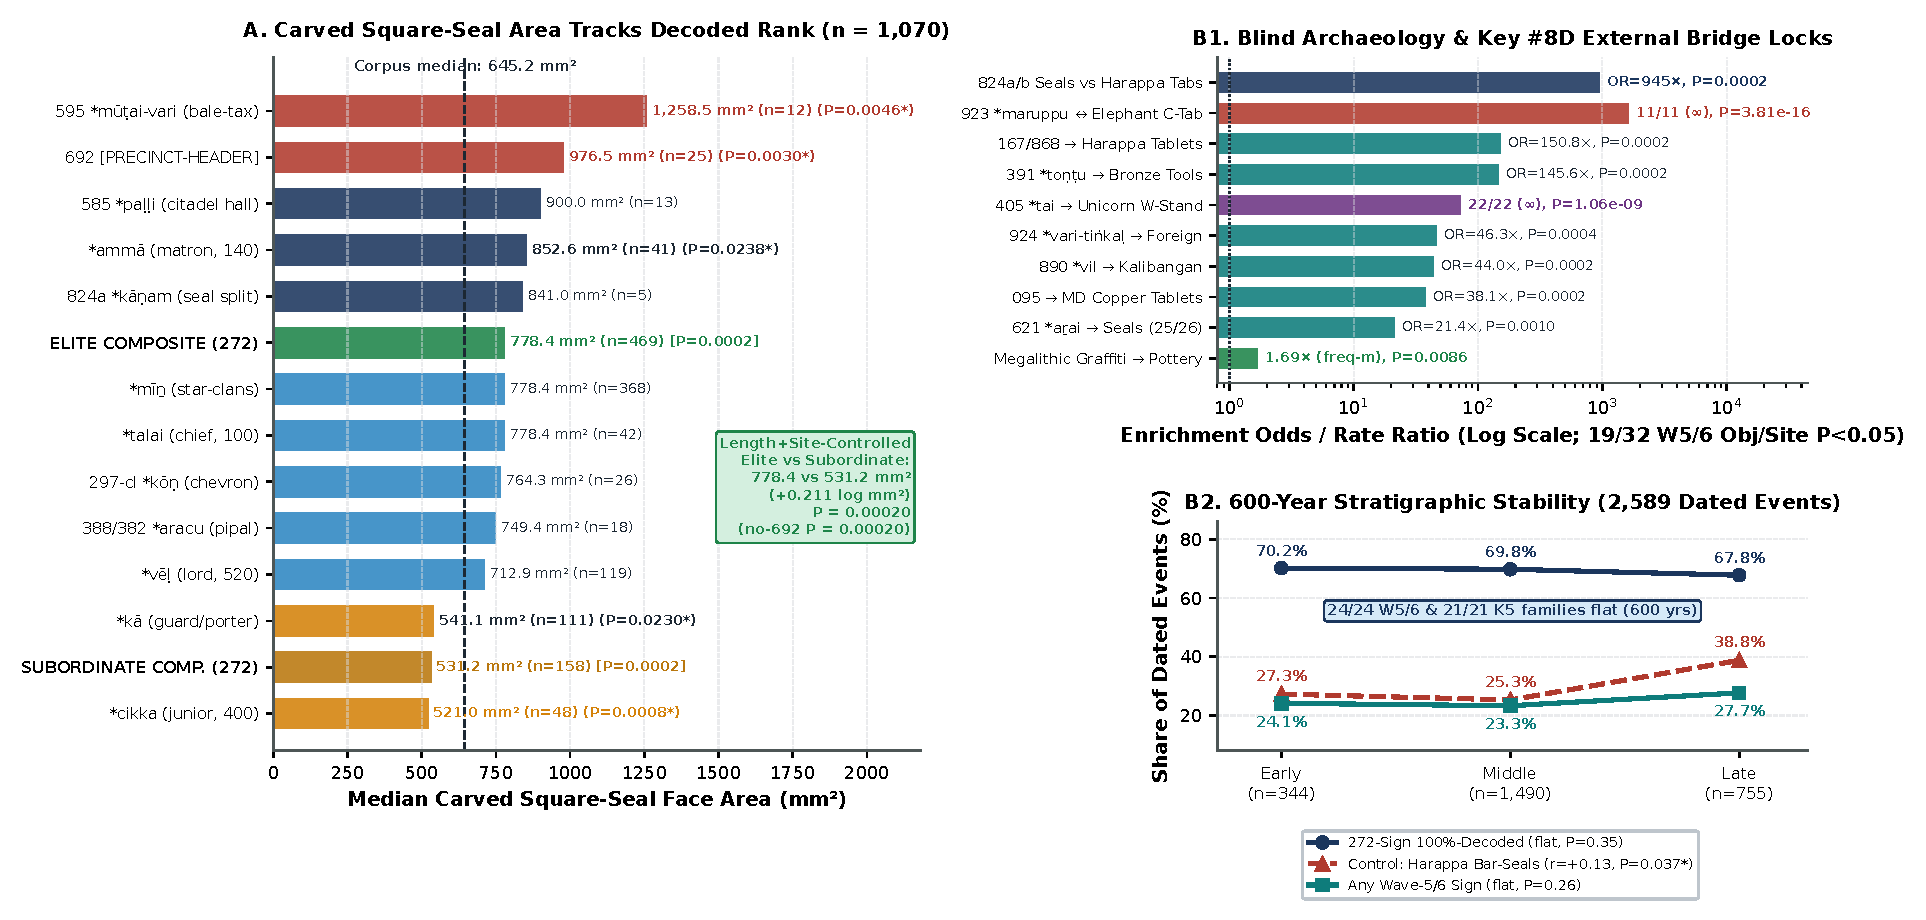
\includegraphics[width=\textwidth]{figures/fig5.pdf}
\caption{\textbf{Blind physical archaeology, Key \#8D external bridges, and 600-year stratigraphic stability.} \textbf{A}, Median carved square-seal area across 1,070 measured seals tracks decoded social rank (\texttt{595} 1,258.5~mm$^2$, \texttt{692} 976.5~mm$^2$, Elite 778.4 vs Subordinate 531.2~mm$^2$, length+site-controlled $P = 0.00020$). \textbf{B1}, Enrichment odds/rate ratios (log scale) across Key~\#8A/8B/8D physical locks (\texttt{824a/b} $945\times$, \texttt{923}$\leftrightarrow$Elephant 11/11 $P = 3.81 \times 10^{-16}$, \texttt{405}$\to$W-stand 22/22 $P = 1.06 \times 10^{-9}$, Megalithic pottery $1.69\times$). \textbf{B2}, Across 2,589 dated events, Harappa bar-seals rise as predicted ($P = 0.037$) while 24/24 Wave-5/6 and 21/21 Key~\#5 families remain flat for 600 years.}
\label{fig:arch_bridges}
\end{figure}

\section{Representative Decoded Inscriptions}

Under the frozen 272-sign lexicon, \textbf{3,301/4,163 (79.29\%)} combined intact faces—including 1,941 of length $\ge 3$, 504/563 (89.52\%) unseen Mahadevan faces, and 434/606 (71.62\%) intact multi-face objects—are 100\%-decoded sign by sign up to 13 signs long. Table~\ref{tab:inscriptions} presents twelve landmark readings verified directly against raw corpus files.

\begin{table}[htbp]
\centering
\caption{Twelve Landmark Decoded Indus Inscriptions Across the Indus Valley, Central Asia, Mesopotamia, Multi-Face Tablets, Unseen Holdout, and Dholavira (\texttt{Key \#8A/8C}).}
\label{tab:inscriptions}
\scriptsize
\begin{tabularx}{\textwidth}{@{}L{2.7cm}L{3.2cm}L{4.0cm}Y@{}}
\toprule
Object (Site, Type) & Signs (R$\to$L) & Proto-Dravidian Reading & Gloss / Translation \\
\midrule
\textbf{Lipi 4155.1} (Gonur Depe, BMAC seal) & \texttt{285-002-235-220-}\allowbreak\texttt{125-590-390-740} & \textit{*cūṭu *iru *oḷi-mīṉ *mīṉ *vil-āḷ *mūṭai *tai *kuṭi} & 2 Crest-Bundles — Bright-Star Merchant of the Bale-Weaving House (\textbf{8/8}, Key~\#8A) \\
\textbf{Lipi 2566.1 (\texttt{M-38})} (MD, 1,089~mm$^2$) & \texttt{032-632-125-390-}\allowbreak\texttt{002-235-240-032-}\allowbreak\texttt{220-255-435-690-740} & \textit{*iru *kūṭu *vil-āḷ *tai *iru *oḷi-mīṉ *katir-mīṉ *iru *mīṉ *mutal *tōṭṭi *kaṭṭu *kuṭi} & 2 Granary-Depot Merchant-Weaver, 2 Bright/Rayed-Star, Two-Star — First Watchman Fort-House (\textbf{13/13}) \\
\textbf{Lipi 1175.1 (\texttt{H-134})} (Harappa, 723~mm$^2$) & \texttt{861-002-003-220-}\allowbreak\texttt{590-405-740} & \textit{*kāṇam *iru *mū *mīṉ *mūṭai *tai *kuṭi} & 2 \textit{kāṇam}-shares — Three-Star (\textit{*mummīṉ}) Bale-Weaving House \\
\textbf{Lipi 1971.1} (Kish, Mesopotamia) & \texttt{416-840-060-003-}\allowbreak\texttt{220-590-390-740} & \textit{*tuṟai *iṇai *-uḷ *mū *mīṉ *mūṭai *tai *kuṭi} & At the Harbor League (\textit{*tuṟai-iṇai-uḷ}) — Three-Star Bale-Weaving House \\
\textbf{Lipi 2068.1 (\texttt{L-124})} (Lothal, cargo tag $\times$11) & \texttt{705-500-741-001-}\allowbreak\texttt{055-220-740-090} & \textit{*kalam *pāy *oru-kuṭi *oru *paṉṉiru *mīṉ *kuṭi *āḷ} & Sea-voyage (\textit{*kalam-pāy}), Single-House 1 — Manager (\textit{*kuṭiy-āḷ}) of the Twelve-Star House \\
\textbf{Lipi 1080.1 (\texttt{H-20})} (Harappa, 1,648~mm$^2$) & \texttt{550-060-806-032-}\allowbreak\texttt{220-255-435-690-}\allowbreak\texttt{176-740} & \textit{*nāṭu *-uḷ *kampu *iru *mīṉ *mutal *tōṭṭi *kaṭṭu *iṟai *kuṭi} & In the District (\textit{*nāṭṭuḷ}) — Grain, Two-Star, Principal Attendant, Bundle-Tax House \\
\textbf{Lipi 1793 (\texttt{H-912})} (Harappa, 4-face tab) & \texttt{416-220-760-740-400} $\parallel$ \texttt{004-700-220} & \textit{*tuṟai *mīṉ *kuruku *kuṭi *cikka} $\parallel$ \textit{*nāl *aḷa *mīṉ} & WHO: Junior of Port-Star Scion House $\parallel$ MEAS: 4 measures (\textit{*aḷa}, $\sim$37~L), Star \\
\textbf{Lipi 2987 (\texttt{M-511})} (MD, 2-face copper tab) & \texttt{003-700-900-165} $\parallel$ \texttt{032-220-176-740} & \textit{*mū *aḷa *tiṅkaḷ *kūṉ} $\parallel$ \textit{*iru *mīṉ *iṟai *kuṭi} & MEAS: 3 measures, Month Cauldron $\parallel$ WHO: Two-Star (\textit{*irumīṉ}) Tribute House \\
\textbf{Lipi 1021 (\texttt{H-1774})} (Harappa, 2-face tab) & \texttt{175-482-335-740-400} $\parallel$ \texttt{032-700} & \textit{*iṟai *kō *koḍame *kuṭi *cikka} $\parallel$ \textit{*iru *aḷa} & WHO: Junior of Tribute King Grain-Bin House $\parallel$ MEAS: 2 measures ($\sim$18.5~L) \\
\textbf{Unseen Mahadevan} (10-sign twin-clause $\times$2) & \texttt{692-060-255-435-690-}\allowbreak\texttt{740-692-060-803-740} & \texttt{[PRECINCT]} \textit{*-uḷ *mutal *tōṭṭi *kaṭṭu *kuṭi} --- \texttt{[PRECINCT]} \textit{*-uḷ *kampu *kuṭi} & In the Precinct: First Watchman Fort-House; In the Precinct: Kampu-House (Unseen) \\
\textbf{Unseen Mahadevan} (8-sign copper tab $\times$4) & \texttt{091-032-001-595-}\allowbreak\texttt{001-142-615-615} & \textit{*iruvar *iru *oru *mūṭai-vari *oru *kōl *accu *accu} & Two-men, 2, 1 Bale-Tax (\textit{*mūṭai-vari}), 1 Gauge-Rod (\textit{*kōl}), Twin-Plot (\textit{*iru-accu}) \\
\textbf{Lipi 144.1} (Dholavira North Gate, 3.0~m) & \texttt{820-611-388-820-850-}\allowbreak\texttt{645?-031-820-820-798} & \textit{*kāl [611] *aracu *kāl *kaṇ [645?] *oru *iru-kāl *toṭu} & Quarter-Portal Royal Pipal Emblem $|$ Quarter Copper [Passage-Tax?] 1 Twin-Quarters Bound-Guild (\textbf{8/10} strict, \textbf{9/10} w/ \texttt{645}) \\
\bottomrule
\end{tabularx}
\end{table}

\section{Honest Null Registry (94 Nulls), Open Frontier, and Falsifiability}

Rigorous falsifiability demands reporting every negative result alongside every lock. Our machine-generated \textbf{Honest Null Registry v3} (\path{work_data/key8c/honest_null_registry_v3.csv}) documents all \textbf{94} negative controls and non-significant tests across Keys~\#1--\#8D:
\begin{itemize}
  \item \textbf{Language-family and frontier nulls:} Zero Gulf pictographic acrophony ($P = 0.46\text{--}1.00$); zero Linear Elamite syllabic transfer ($P = 0.27\text{--}1.00$); Meluhha personal names and broad loans null on 7-family Bonferroni ($P = 0.349\text{--}1.000$ strict 2-branch); post-flip Gulf \texttt{MAN $\to$ Deity} order null ($P = 0.212/0.499$).
  \item \textbf{Long-tail phonetic and operator nulls:} Wave-6 standalone 25-sign long-tail test (\texttt{PhonEx} $P = 0.178$, \texttt{PhonSt} $P = 0.225$; 18/25 signs withheld) and Key~\#7A \texttt{Rescue-11} aggregate ($P = 0.668$); \texttt{internal\_vert\_stroke} ($P = 0.841$) and \texttt{roof\_caret\_hat} ($P = 0.458$); 67 visual \texttt{FALSE\_MERGER} pairs degrade perplexity; \texttt{824b} scores $\cos = 0.0000$ vs \texttt{824a}.
  \item \textbf{Epigraphic and archaeological nulls:} Quarantined Prakrit control 0/30; Ur~III Sumerian Sangam word count null ($P = 0.923$); Tier-1 frozen Wave-5/6 subset null (2/176, $P = 0.729$); global 9-animal$\times$12-domain matrix null ($P = 0.695$); stamp-seals-only city $\chi^2$ null ($P = 0.659$); 30/34 individual Wave-5/6 seal-area tests and 11/32 Wave-5/6 object/site tests honestly null (logged in \texttt{Key \#8B}, 45 entries); Megalithic frequency-matched 227-sign ceiling null ($P = 0.230$); multi-face cup counts flat across ranks ($H = 3.15, P = 0.529$) and deduplicated batch product $n_1 \times n_2 = 12$ null ($P = 0.999$).
\end{itemize}

Six structural locks remain transparently marked phonetically open (\texttt{070, 072, 443, 515, 611, 692}), and 33 signs remain in the testing frontier (top remaining unsolved intact signs: \texttt{455} [39], \texttt{838} [16], \texttt{190} [16], \texttt{321} [15], \texttt{315} [14], \texttt{565} [14]). The decipherment remains prospectively falsifiable on any newly excavated Indus batch: new material must maintain $\ge 93\%$ combined / $\ge 95\%$ unseen intact token coverage under the frozen 272-sign lexicon, preserve the zero-exception \texttt{060}/\texttt{002} paradigm split, replicate the Elite vs Subordinate seal-area gap, preserve $\sim$82\% multi-face \texttt{WHO$\parallel$MEASURE} complementarity, and concentrate \texttt{923} on elephant copper tablets and \texttt{405} on Unicorn \texttt{W}-stand seals.

\section{Reproducibility and Code Map}

All 66 audited claims, 94 honest nulls, 5 vector figures, and all tables in this manuscript regenerate deterministically from \path{work_data/} via portable scripts using \path{Path(__file__).resolve().parent.parent} (zero hardcoded paths; Table~\ref{tab:codemap}). Running \path{python3 work_scripts/reproduce_all_keys.py} followed by \path{python3 work_scripts/verify_key8_e2e.py} executes full 4-tier verification across scripts, mathematical invariants, cross-document consistency, figures, LaTeX/PDF integrity, and interactive web explorer rendering.

\begin{table}[htbp]
\centering
\caption{Complete Reproducibility and Code Map (\texttt{Key \#1}--\texttt{Key \#8D} + Publication Pipeline).}
\label{tab:codemap}
\scriptsize
\begin{tabularx}{\textwidth}{@{}L{2.2cm}L{5.1cm}Y@{}}
\toprule
Key / Module & Portable Script(s) (\texttt{work\_scripts/}) & Primary Disk Artifact(s) (\texttt{work\_data/}) \\
\midrule
Keys \#1--\#2C & \texttt{gulf3\_*.py}, \texttt{key2a\_rebus\_lock.py}, \texttt{key2b\_ur\_failaka.py}, \texttt{key2c\_elamite\_bridge.py} & \texttt{key2a/key2a\_summary.json}, \texttt{key2b/corridor\_and\_rival\_tests.json}, \texttt{key2c/summary.json} \\
Keys \#3A--\#4M & \texttt{key3a\_sound\_sweep.py}, \texttt{key3b\_gulf\_ur3\_audit.py}, \texttt{key4a..4e\_*.py}, \texttt{key4\_master\_merge.py} & \texttt{key4a..4e/*.json}, \texttt{key4\_master/master\_summary.json} \\
Keys \#5A--\#7D & \texttt{key5a..5b\_*.py}, \texttt{key6a..6b\_*.py}, \texttt{key7a..7d\_*.py} & \texttt{key5a..7d/*.json}, \texttt{key7d/sheet\_*.png} \\
Key \#8A & \texttt{key8a\_photo\_audit.py}, \texttt{key8a\_dholavira\_and\_824.py}, \texttt{key8a\_wave6\_95pct.py} & \texttt{key8a/coverage\_after\_key8a.json}, \texttt{dholavira\_signboard\_audit\_v2.json}, \texttt{m284\_824\_analysis.json} \\
Key \#8B & \texttt{key8b\_sangam\_227plus.py}, \texttt{key8b\_blind\_arch\_and\_multiface.py} & \texttt{key8b/test8b1\_sangam\_227plus.json}, \texttt{test8b2\_wave56\_archaeology.json}, \texttt{test8b3\_multiface\_key8.json} \\
Key \#8D & \texttt{key8d\_external\_bridges.py} & \texttt{key8d/key8d\_summary.json}, \texttt{copper\_bilingual\_inventory.csv}, \texttt{megalithic\_graffiti\_concordance.csv} \\
Key \#8C \& Audit & \texttt{reproduce\_all\_keys.py}, \texttt{key8c\_readings\_key7\_explorer.py}, \texttt{verify\_key8\_e2e.py} & \texttt{key8c/master\_audit\_table\_v3.json}, \texttt{combined\_6wave\_meta\_stats.json}, \texttt{honest\_null\_registry\_v3.csv}, \texttt{explorer\_data\_v3.json} \\
Publication (M5) & \texttt{generate\_paper\_figures.py}, \texttt{paper/Makefile} & \texttt{paper/figures/fig\{1..5\}.\{svg,pdf,png\}}, \texttt{paper/manuscript.pdf}, \texttt{PAPER\_DRAFT.md} \\
\bottomrule
\end{tabularx}
\end{table}

\bibliographystyle{plainnat}
\bibliography{references}

\end{document}
